\documentclass{beamer}

% xcolor and define colors -------------------------
\usepackage{xcolor}

% https://www.viget.com/articles/color-contrast/
\definecolor{purple}{HTML}{5601A4}
\definecolor{navy}{HTML}{0D3D56}
\definecolor{ruby}{HTML}{9a2515}
\definecolor{alice}{HTML}{107895}
\definecolor{daisy}{HTML}{EBC944}
\definecolor{coral}{HTML}{F26D21}
\definecolor{kelly}{HTML}{829356}
\definecolor{cranberry}{HTML}{E64173}
\definecolor{jet}{HTML}{131516}
\definecolor{asher}{HTML}{555F61}
\definecolor{slate}{HTML}{314F4F}

% Mixtape Sessions
\definecolor{picton-blue}{HTML}{00b7ff}
\definecolor{violet-red}{HTML}{ff3881}
\definecolor{sun}{HTML}{ffaf18}
\definecolor{electric-violet}{HTML}{871EFF}

% Main theme colors
\definecolor{accent}{HTML}{00b7ff}
\definecolor{accent2}{HTML}{871EFF}
\definecolor{gray100}{HTML}{f3f4f6}
\definecolor{gray800}{HTML}{1F292D}


% Beamer Options -------------------------------------

% Background
\setbeamercolor{background canvas}{bg = white}

% Change text margins
\setbeamersize{text margin left = 15pt, text margin right = 15pt} 

% \alert
\setbeamercolor{alerted text}{fg = accent2}

% Frame title
\setbeamercolor{frametitle}{bg = white, fg = jet}
\setbeamercolor{framesubtitle}{bg = white, fg = accent}
\setbeamerfont{framesubtitle}{size = \small, shape = \itshape}

% Block
\setbeamercolor{block title}{fg = white, bg = accent2}
\setbeamercolor{block body}{fg = gray800, bg = gray100}

% Title page
\setbeamercolor{title}{fg = gray800}
\setbeamercolor{subtitle}{fg = accent}

%% Custom \maketitle and \titlepage
\setbeamertemplate{title page}
{
    %\begin{centering}
        \vspace{20mm}
        {\Large \usebeamerfont{title}\usebeamercolor[fg]{title}\inserttitle}\\
        {\large \itshape \usebeamerfont{subtitle}\usebeamercolor[fg]{subtitle}\insertsubtitle}\\ \vspace{10mm}
        {\insertauthor}\\
        {\color{asher}\small{\insertdate}}\\
    %\end{centering}
}

% Table of Contents
\setbeamercolor{section in toc}{fg = accent!70!jet}
\setbeamercolor{subsection in toc}{fg = jet}

% Button 
\setbeamercolor{button}{bg = accent}

% Remove navigation symbols
\setbeamertemplate{navigation symbols}{}

% Table and Figure captions
\setbeamercolor{caption}{fg=jet!70!white}
\setbeamercolor{caption name}{fg=jet}
\setbeamerfont{caption name}{shape = \itshape}

% Bullet points

%% Fix left-margins
\settowidth{\leftmargini}{\usebeamertemplate{itemize item}}
\addtolength{\leftmargini}{\labelsep}

%% enumerate item color
\setbeamercolor{enumerate item}{fg = accent}
\setbeamerfont{enumerate item}{size = \small}
\setbeamertemplate{enumerate item}{\insertenumlabel.}

%% itemize
\setbeamercolor{itemize item}{fg = accent!70!white}
\setbeamerfont{itemize item}{size = \small}
\setbeamertemplate{itemize item}[circle]

%% right arrow for subitems
\setbeamercolor{itemize subitem}{fg = accent!60!white}
\setbeamerfont{itemize subitem}{size = \small}
\setbeamertemplate{itemize subitem}{$\rightarrow$}

\setbeamertemplate{itemize subsubitem}[square]
\setbeamercolor{itemize subsubitem}{fg = jet}
\setbeamerfont{itemize subsubitem}{size = \small}

% Special characters

\usepackage{collectbox}

\makeatletter
\newcommand{\mybox}{%
    \collectbox{%
        \setlength{\fboxsep}{1pt}%
        \fbox{\BOXCONTENT}%
    }%
}
\makeatother






% Links ----------------------------------------------

\usepackage{hyperref}
\hypersetup{
  colorlinks = true,
  linkcolor = accent2,
  filecolor = accent2,
  urlcolor = accent2,
  citecolor = accent2,
}


% Line spacing --------------------------------------
\usepackage{setspace}
\setstretch{1.2}


% \begin{columns} -----------------------------------
\usepackage{multicol}


% Fonts ---------------------------------------------
% Beamer Option to use custom fonts
\usefonttheme{professionalfonts}

% \usepackage[utopia, smallerops, varg]{newtxmath}
% \usepackage{utopia}
\usepackage[sfdefault,light]{roboto}

% Small adjustments to text kerning
\usepackage{microtype}



% Remove annoying over-full box warnings -----------
\vfuzz2pt 
\hfuzz2pt


% Table of Contents with Sections
\setbeamerfont{myTOC}{series=\bfseries, size=\Large}
\AtBeginSection[]{
        \frame{
            \frametitle{Roadmap}
            \tableofcontents[current]   
        }
    }


% Tables -------------------------------------------
% Tables too big
% \begin{adjustbox}{width = 1.2\textwidth, center}
\usepackage{adjustbox}
\usepackage{array}
\usepackage{threeparttable, booktabs, adjustbox}
    
% Fix \input with tables
% \input fails when \\ is at end of external .tex file
\makeatletter
\let\input\@@input
\makeatother

% Tables too narrow
% \begin{tabularx}{\linewidth}{cols}
% col-types: X - center, L - left, R -right
% Relative scale: >{\hsize=.8\hsize}X/L/R
\usepackage{tabularx}
\newcolumntype{L}{>{\raggedright\arraybackslash}X}
\newcolumntype{R}{>{\raggedleft\arraybackslash}X}
\newcolumntype{C}{>{\centering\arraybackslash}X}

% Figures

% \imageframe{img_name} -----------------------------
% from https://github.com/mattjetwell/cousteau
\newcommand{\imageframe}[1]{%
    \begin{frame}[plain]
        \begin{tikzpicture}[remember picture, overlay]
            \node[at = (current page.center), xshift = 0cm] (cover) {%
                \includegraphics[keepaspectratio, width=\paperwidth, height=\paperheight]{#1}
            };
        \end{tikzpicture}
    \end{frame}%
}

% subfigures
\usepackage{subfigure}


% Highlight slide -----------------------------------
% \begin{transitionframe} Text \end{transitionframe}
% from paulgp's beamer tips
\newenvironment{transitionframe}{
    \setbeamercolor{background canvas}{bg=accent!40!black}
    \begin{frame}\color{accent!10!white}\LARGE\centering
}{
    \end{frame}
}


% Table Highlighting --------------------------------
% Create top-left and bottom-right markets in tabular cells with a unique matching id and these commands will outline those cells
\usepackage[beamer,customcolors]{hf-tikz}
\usetikzlibrary{calc}
\usetikzlibrary{fit,shapes.misc}

% To set the hypothesis highlighting boxes red.
\newcommand\marktopleft[1]{%
    \tikz[overlay,remember picture] 
        \node (marker-#1-a) at (0,1.5ex) {};%
}
\newcommand\markbottomright[1]{%
    \tikz[overlay,remember picture] 
        \node (marker-#1-b) at (0,0) {};%
    \tikz[accent!80!jet, ultra thick, overlay, remember picture, inner sep=4pt]
        \node[draw, rectangle, fit=(marker-#1-a.center) (marker-#1-b.center)] {};%
}

\usepackage{breqn} % Breaks lines

\usepackage{amsmath}
\usepackage{mathtools}

\usepackage{pdfpages} % \includepdf

\usepackage{listings} % R code
\usepackage{verbatim} % verbatim

% Video stuff
\usepackage{media9}

% packages for bibs and cites
\usepackage{natbib}
\usepackage{har2nat}
\newcommand{\possessivecite}[1]{\citeauthor{#1}'s \citeyearpar{#1}}
\usepackage{breakcites}
\usepackage{alltt}

% tikz
\usepackage{tikz}
\usepackage{pgfplots}
\usetikzlibrary{calc, positioning, decorations.pathreplacing, arrows.meta, intersections}
\pgfdeclarelayer{bg}
\pgfdeclarelayer{back}
\pgfdeclarelayer{fg}
\pgfsetlayers{bg,main,fg,back}
\usetikzlibrary{shapes,arrows}

% Setup math operators
\DeclareMathOperator{\E}{E} \DeclareMathOperator{\tr}{tr} \DeclareMathOperator{\se}{se} \DeclareMathOperator{\I}{I} \DeclareMathOperator{\sign}{sign} \DeclareMathOperator{\supp}{supp} \DeclareMathOperator{\plim}{plim}
\DeclareMathOperator*{\dlim}{\mathnormal{d}\mkern2mu-lim}
\newcommand\independent{\protect\mathpalette{\protect\independenT}{\perp}}
   \def\independenT#1#2{\mathrel{\rlap{$#1#2$}\mkern2mu{#1#2}}}
\newcommand*\colvec[1]{\begin{pmatrix}#1\end{pmatrix}}

\newcommand{\myurlshort}[2]{\href{#1}{\textcolor{gray}{\textsf{#2}}}}


\begin{document}

\imageframe{./lecture_includes/mixtape_ci_cover.png}


% ---- Content ----


\section{Directed Acyclic Graphs}

\begin{frame}{Double De-biased Machine Larning}

\begin{itemize}

\item This is an important paper.  It's by Chernozhukov, et al. (2018) and has been very influential
\item But the elements of it are found in ideas that I think we have to cover because otherwise the technical mechanics of it will overshadow important parts that I think you can't skip
\item DML, as I'll call it, ultimately is a machine learning based method for handling a large number of variables (features) to reconstruct counterfactuals
\item But these variables still cannot just be haphazardly selected and we need to see why -- there are no magic wands in causal inference sadly

\end{itemize}

\end{frame}

\begin{frame}{Control for X}

\begin{itemize}

\item The easiest way to motivate the core identifying assumptions for DML is to start with graphs
\item Then move into regression and explain the concepts of curse of dimensionality and why contemporary data sources swamp our matching estimators
\item We rely therefore on extrapolation using penalized regressions and other ML methods, but these are still just "control for $X$"

\end{itemize}

\end{frame}

\begin{frame}{Adjusting for variables}

\begin{itemize}
\item One of the first things you learn in a methods course is multivariate regression ``controlling for $X$''
\item What is this? Why do we do this?  What should $X$ be? What causal parameter does it help identify?
\item Unconfoundedness, selection on observables, ignorable treatment assignment are different terms describing the same thing -- the RCT is still occurring, only within the dimensions of a conditioning set of confounders and covariates
\end{itemize}

\end{frame}



\begin{frame}{Judea Pearl and DAGs}


  \begin{itemize}
    \item As you maybe know, Judea Pearl and colleagues in Artificial Intelligence at UCLA developed DAG modeling to create a formalized causal inference methodology
    \item We will only focus on one idea called the backdoor criterion and link that to unconfoundedness, a potential outcomes framework that underlies the DML estimator
    \item I will be emphasizing things that others don't emphasize when introducing DML, but that is just my style
  \end{itemize}

\end{frame}


\begin{frame}{Further reading}

  \begin{enumerate}

	\item Molak (2023), \underline{Causal Inference and Discovery in Python} (good)
	\item Facure (2023), \underline{Causal Inference in Python: Applying Causal Inference in the Tech Industry} (great)
	\item Facure (2022) \underline{Causal Inference for the Brave and the Bold} (also fantastic)
	\item Brigham Frandsen's online workshops which I'll share for free
	
  \end{enumerate}

\end{frame}

\begin{frame}{Design vs. Model}

  \begin{itemize}
    \item DAGs are way too tempting in my opinion, and I think they may take us backwards a little, but they are core parts of modern causal inference mapping onto ML, and in particular tech
	\item They are extremely helpful for thinking through the differences between good and bad controls, which DML will not be able to differentiate
  \end{itemize}

\end{frame}



\begin{frame}{Causal model}

  \begin{itemize}
    \item The causal model is sometimes called the structural model, but for us, I prefer the former as it's less alienating
    \item It's the system of equations describing the relevant aspects of the world
    \item It necessarily is filled with causal effects associated with some particular comparative statics
    \item Consider the following diagram representing the returns to education with simplified confounders
  \end{itemize}

\end{frame}

\begin{frame}[plain]

  \begin{center}
    \begin{tikzpicture}[node distance=1.5cm]
      % nodes %
      \node[text centered] (d) {$D$};
      \node[right of = d, text centered] (y) {$Y$};
      \node[above left of = d, text centered] (i) {$I$};
      \node[left of = i, text centered] (pe) {$PE$};
      \node[below of = pe, text centered] (b) {$B$};
      % edges %
      \draw[->, line width= 1] (d) -- (y);
      \draw[->, line width= 1,] (i) -- (d);
      \draw[->, line width= 1,] (pe) -- (i);
      \draw[->, line width= 1,] (pe) -- (d);
      \draw[->, line width= 1, dashed] (b) -- (pe);
      \draw[->, line width= 1, dashed] (b) -- (d);
      \draw[->, line width= .5] (i) to [out=45,in=135, looseness=0.5] (y);
    \end{tikzpicture}
  \end{center}

  \bigskip
  \begin{itemize}
    \item $B$ is a \textbf{parent} of $PE$ and $D$
    \item $PE$ and $D$ are \textbf{descendants} of $B$
    \item There is a \textbf{direct (causal) path} from $D$ to $Y$
    \item There is a \textbf{mediated (causal) path} from $B$ to $Y$ through $D$
    \item There are six \textbf{paths} from $PE$ to $Y$ but none are direct, but some of them are different in other ways
  \end{itemize}
\end{frame}





\begin{frame}{Where do DAGs come from?}

	\begin{itemize}
	\item DAGs are meant to represent ``contemporary agreement among experts'' -- if you aren't willing to present your DAG before a room of experts, it's likely you shouldn't use it at all
	\item But more than that, the DAG is a local graph -- it's the modeling of the treatment assignment mechanism in your local context, not merely some model of monopolies or whateer
	\item Your DAG should be a reasonable approximation of $D$ and $Y$ parents (confounders) and direct and indirect effects of $D$ on $Y$
	\item We get ideas for DAGs from theory, models, observation, experience, prior studies, intuition, as well as conversations with domain experts
	\end{itemize}

\end{frame}

% 	\item The DAG is a reasonable approximation of all common parents of $D$ and $Y$ (confounders) and direct relationships between $D and $Y$


\subsection{Backdoor criterion}

\begin{frame}{Unconfoundedness and the backdoor criterion}

  \begin{itemize}

    \item DAGs help us understand the source of problems in our observational (non-experimental) data that make inferring causality hard
    \item But it also can help us see a way out in some situations
    \item We will focus today on the unconfoundedness research design, which is best described in causal graphs with the concept of the \textbf{backdoor criterion}
    \item As we will see, the DAG helps you solve the problem of choosing covariates for a model to resolve selection bias, but to do so requires confidence in your DAG
  \end{itemize}

\end{frame}

\begin{frame}{Confounding}

  \begin{itemize}
    \item Confounding occurs when when the treatment and the outcomes have a common parent node as that creates spurious correlation between $D$ and $Y$

          \begin{center}
            \begin{tikzpicture}
              [node distance=1.5cm]
              % nodes %
              \node[text centered] (d) {$D$};
              \node[below right of = d, text centered] (x) {$X$};
              \node[above right of = x, text centered] (y) {$Y$};

              % edges %
              \draw[->, line width= 1] (d) -- (y);
              \draw[->, line width= 1] (x) -- (d);
              \draw[->, line width= 1] (x) -- (y);
            \end{tikzpicture}
          \end{center}

          \item Confounders are causing selection bias $E[Y^0|D=1, X] \neq E[Y^0|D=0, X]$ due to differences in $X$ which are shaping $Y^0$ differentially by treatment status
  \end{itemize}
\end{frame}

\begin{frame}{Backdoor Paths}

  \begin{itemize}
    \item Confounding creates \textbf{backdoor paths} between treatment and outcome ($D\leftarrow X\rightarrow Y$) -- i.e., spurious correlations
		\begin{itemize}
		\item Distinct from something called a collider path ($D \rightarrow X \leftarrow Y$)
		\item Distinct from something called a mediator path ($D \rightarrow X \rightarrow Y$)
		\end{itemize}
    \item We can ``block'' any particular backdoor path by conditioning on variable $X$ so long as it is not a collider (visualized here with a square over X)

  \end{itemize}

  \begin{center}
    \begin{tikzpicture}
      [node distance=1.5cm]
      % nodes %
      \node[text centered] (d) {$D$};
      \node[below right of = d, text centered, rectangle, draw, thin] (x) {$X$};
      \node[above right of = x, text centered] (y) {$Y$};

      % edges %
      \draw[->, line width= 1] (d) -- (y);
      \draw[->, line width= 1] (x) -- (d);
      \draw[->, line width= 1] (x) -- (y);
    \end{tikzpicture}
  \end{center}

\end{frame}

\begin{frame}{Backdoor Paths}

  \begin{itemize}
    \item Once we condition on $X$, we can calculate average differences in $Y$ by treatment status to obtain an estimate of an aggregate causal parameter
    \item There are many methods for doing this and we cover them today -- regression, matching, stratification, weights
    \item But all of them at their fundamental level are calculating simple differences in mean outcomes for given values of $X$ and then taking weighted averages

  \end{itemize}

  \begin{center}
    \begin{tikzpicture}
      [node distance=1.5cm]
      % nodes %
      \node[text centered] (d) {$D$};
      \node[below right of = d, text centered, rectangle, draw, thin] (x) {$X$};
      \node[above right of = x, text centered] (y) {$Y$};

      % edges %
      \draw[->, line width= 1] (d) -- (y);
      \draw[->, line width= 1] (x) -- (d);
      \draw[->, line width= 1] (x) -- (y);
    \end{tikzpicture}
  \end{center}

\end{frame}


\begin{frame}{Backdoor Paths}

  \begin{itemize}

	\item When all backdoor paths from $D$ to $Y$ are blocked, then the only remaining path between $D$ to $Y$ is the causal path
	\item We call this satisfying the backdoor criterion using Pearl's DAG terminology, and we call it unconfoundedness using Rubin's potential outcomes terminology (which I'll discuss later)

  \end{itemize}

  \begin{center}
    \begin{tikzpicture}
      [node distance=1.5cm]
      % nodes %
      \node[text centered] (d) {$D$};
      \node[below right of = d, text centered, rectangle, draw, thin] (x) {$X$};
      \node[above right of = x, text centered] (y) {$Y$};

      % edges %
      \draw[->, line width= 1] (d) -- (y);
      \draw[->, line width= 1] (x) -- (d);
      \draw[->, line width= 1] (x) -- (y);
    \end{tikzpicture}
  \end{center}

\end{frame}








\begin{frame}{Backdoor criterion}


  \begin{block}{Backdoor criterion}
    Conditioning on $X$ satisfies the backdoor criterion with respect to $(D,Y)$ directed path if:
    \begin{enumerate}
      \item All backdoor paths are blocked by $X$
      \item No element of $X$ is a collider

    \end{enumerate}

    
  \end{block}
       Conditioning on a non-collider is sufficient to closing a backdoor path even if it's been opened by conditioning on a collider, so just be sure to close a backdoor path if you opened it with a collider


\end{frame}

\begin{frame}{What control strategy meets the backdoor criterion?}
  \begin{itemize}
    \item List all backdoor paths from $D$ to $Y$. I'll wait.

          \begin{center}
            \begin{tikzpicture}
              [node distance=1.5cm]
              % nodes %
              \node[text centered,rectangle,thin] (x1) {$X_1$};
              \node[right of = x1, text centered] (d) {$D$};
              \node[below right of = d, text centered] (x2) {$X_2$};
              \node[above right of = x2, text centered] (y) {$Y$};

              % edges %
              \draw[->, line width= .5] (x1) -- (d);
              \draw[->, line width= .5] (d) -- (y);
              \draw[->, line width= .5] (x2) -- (d);
              \draw[->, line width= .5] (x2) -- (y);
              \draw[->, line width= .5] (x1) to [out=45,in=135, looseness=0.5] (y);
            \end{tikzpicture}
          \end{center}

    \item What are the necessary and sufficient set of controls which will satisfy the backdoor criterion?
  \end{itemize}

  \framebreak




\end{frame}


\begin{frame}{What if you have an unobservable?}


  \begin{itemize}
    \item List all the backdoor paths from $D$ to $Y$.

          \begin{center}
            \begin{tikzpicture}
              [node distance=1.5cm]
              % nodes %
              \node[text centered] (u) {$U$};
              \node[right of = u, text centered] (x2) {$X_2$};
              \node[above of = x2, text centered] (x1) {$X_1$};
              \node[right of = x2, text centered] (d) {$D$};
              \node[right of = d, text centered] (y) {$Y$};

              % edges %
              \draw[->, line width= .5, dashed] (u) -- (x2);
              \draw[->, line width= .5] (x2) -- (d);
              \draw[->, line width= .5] (x1) -- (d);
              \draw[->, line width= .5] (x1) -- (y);
              \draw[->, line width= .5] (d) -- (y);
              \draw[->, line width= .5, dashed] (u) to [out=-45,in=-135, looseness=0.5] (y);
            \end{tikzpicture}
          \end{center}

    \item What are the necessary and sufficient set of controls which will satisfy the backdoor criterion?
    \item What about the unobserved variable, $U$?
  \end{itemize}

  \framebreak


\end{frame}






\subsection{Collider bias}

\begin{frame}{Collider bias}

\begin{itemize}
\item Backdoor paths can remain open in covariate adjustment strategies through two ways:
	\begin{enumerate}
	\item You did not close the path because you did not condition on the confounder
	\item Your conditioning variable opened up a previously closed backdoor path because on that path the variable was a \textbf{collider}
	\end{enumerate}
\item Colliders are ``bad controls'' which when you control for them, \emph{create} new previously non-existent spurious correlations (not commonly discussed, even in economics)
\item This is the risk of blindly controlling for variables (``kitchen sink regressions'')
\end{itemize}

\end{frame}


\begin{frame}{Example 1: Movie stars}

  \alert{Important}: Since unconditioned colliders block back-door paths, what exactly does conditioning on a collider do? Let's illustrate with a fun example and some made-up data\\
  \begin{itemize}
    \item \underline{CNN.com} headline: Megan Fox voted worst -- but sexiest -- actress of 2009 \myurlshort{http://marquee.blogs.cnn.com/2009/12/30/megan-fox-voted-worst-but-sexiest-actress-of-2009/}{(link)}
    \item Are these two things actually negatively correlated in the world?
    \item Assume talent and beauty are independent, but each causes someone to become a movie star.  What's the correlation between talent and beauty for a sample of movie stars compared to the population as a whole (stars and non-stars)?
  \end{itemize}

\end{frame}


\begin{frame}{Movie star DAG}

Imagine casting directors pick movie stars based on talent and beauty

  \begin{center}
    \begin{tikzpicture}
      [node distance=2cm, text centered]

      %nodes
      \node[text centered,draw,rectangle,thin] (x) {Movie Star};
      \node[below left of = x] (u1) {$Talent$};
      \node[below right of = x] (u2) {$Beauty$};

      % edges %
      \draw[->, line width= 2] (u1) -- (x);
      \draw[->, line width= 2] (u2) -- (x);
    \end{tikzpicture}
  \end{center}

Talent and beauty can become correlated even though they are independent


\end{frame}

\begin{frame}[shrink=20,plain]

  \begin{figure}
    \includegraphics[height=9cm]{./lecture_includes/beauty_collider.pdf}
    \caption{Top left figure: Non-star sample scatter plot of beauty (vertical axis) and talent (horizontal axis). Top right right figure: Star sample scatter plot of beauty and talent.  Bottom left figure: Entire (stars and non-stars combined) sample scatter plot of beauty and talent.}
  \end{figure}
\end{frame}

\begin{frame}{Sample selection?}

\begin{itemize}
\item Notice that this is clear when we are focused on sample selection
\item But even a regression that included ``star'' would create the issue:$$beauty_i = \alpha + \delta talent_i + \beta star_i + \varepsilon_i$$
\item It's not just sample selection 
\end{itemize}

\end{frame}


\begin{frame}[allowframebreaks,plain]

  \begin{itemize}
    \item \textbf{Colliders can be outcomes (and often those are the ones)}
          \begin{itemize}
            \item There is only one backdoor path from $D$ to $Y$

                  \begin{center}
                    \begin{tikzpicture}
                      [node distance=1.5cm]
                      % nodes %
                      \node[text centered,draw,rectangle,thin] (x1) {$X_1$};
                      \node[right of = x1, text centered] (d) {$D$};
                      \node[below right of = d, text centered] (x2) {$X_2$};
                      \node[above right of = x2, text centered] (y) {$Y$};

                      % edges %
                      \draw[->, line width= .5] (x1) -- (d);
                      \draw[->, line width= .5] (d) -- (y);
                      \draw[->, line width= .5] (d) -- (x2);
                      \draw[->, line width= .5] (y) -- (x2);
                      \draw[->, line width= .5] (x1) to [out=45,in=135, looseness=0.5] (y);
                    \end{tikzpicture}
                  \end{center}
                  

            \item Conditioning on $X_1$ blocks the backdoor path


            \item But what if we also condition on $X_2$?

                  \begin{center}
                    \begin{tikzpicture}
                      [node distance=1.5cm]
                      % nodes %
                      \node[text centered,draw,rectangle,thin] (x1) {$X_1$};
                      \node[right of = x1, text centered] (d) {$D$};
                      \node[below right of = d, draw, rectangle, text centered] (x2) {$X_2$};
                      \node[above right of = x2, text centered] (y) {$Y$};

                      % edges %
                      \draw[->, line width= .5] (x1) -- (d);
                      \draw[->, line width= .5] (d) -- (y);
                      \draw[->, line width= .5] (d) -- (x2);
                      \draw[->, line width= .5] (y) -- (x2);
                      \draw[->, line width= .5] (x1) to [out=45,in=135, looseness=0.5] (y);
                    \end{tikzpicture}
                  \end{center}

            \item Conditioning on $X_2$ opens up a new path, creating new spurious correlations between $D$ and $Y$ 
          \end{itemize}

          \framebreak


    \item \textbf{Colliders could be pre-treatment covariates (called M-bias because it looks like an M)}
          \begin{itemize}
            \item Name the backdoor paths.  Is it open or closed?

                  \begin{center}
                    \begin{tikzpicture}
                      [node distance=1.5cm, text centered]
                      % nodes %
                      \node[] (x) {$X$};
                      \node[above left of = x] (u1) {$U_1$};
                      \node[below left of = x] (u2) {$U_2$};
                      \node[right of = x] (d) {$D$};
                      \node[right of = d] (y) {$Y$};

                      % edges %
                      \draw[->, line width= .5, dashed] (u1) -- (x);
                      \draw[->, line width= .5, dashed] (u2) -- (x);
                      \draw[->, line width= .5, dashed] (u1) to [out=0,in=135, looseness=0.5] (y);
                      \draw[->, line width= .5, dashed] (u2) to [out=0,in=-135, looseness=0.5] (d);
                      \draw[->, line width= .5] (d) -- (y);
                    \end{tikzpicture}
                  \end{center}

            \item But what if we condition on $X$?

                  \begin{center}
                    \begin{tikzpicture}
                      [node distance=1.5cm, text centered]
                      % nodes %
                      \node[text centered,draw,rectangle,thin] (x) {$X$};
                      \node[above left of = x] (u1) {$U_1$};
                      \node[below left of = x] (u2) {$U_2$};
                      \node[right of = x] (d) {$D$};
                      \node[right of = d] (y) {$Y$};

                      % edges %
                      \draw[->, line width= .5, dashed] (u1) -- (x);
                      \draw[->, line width= .5, dashed] (u2) -- (x);
                      \draw[->, line width= .5, dashed] (u1) to [out=0,in=135, looseness=0.5] (y);
                      \draw[->, line width= .5, dashed] (u2) to [out=0,in=-135, looseness=0.5] (d);
                      \draw[->, line width= .5] (d) -- (y);
                    \end{tikzpicture}
                  \end{center}


          \end{itemize}
  \end{itemize}
  \framebreak


\end{frame}


\begin{frame}{Testing the Validity of the DAG}

  \begin{itemize}
    \item The DAG makes testable predictions, and there is also new work on ``causal discovery'' which is outside my area of expertise (see Molak and the DoWhy package in python)
    \item Conditional on $D$ and $I$, parental education ($PE$) should no longer be correlated with $Y$
    \item Can be hard to figure this out by hand, but software can help (e.g., Daggity.net is browser based, Causal Fusion is more advanced)
    \item Causal algorithms tend to be DAG based and are becoming popular in industry 
  \end{itemize}

  \begin{center}
    \begin{tikzpicture}[node distance=1.5cm]
      % nodes %
      \node[text centered] (d) {$D$};
      \node[right of = d, text centered] (y) {$Y$};
      \node[above left of = d, text centered] (i) {$I$};
      \node[left of = i, text centered] (pe) {$PE$};
      \node[below of = pe, text centered] (b) {$B$};
      % edges %
      \draw[->, line width= 1] (d) -- (y);
      \draw[->, line width= 1,] (i) -- (d);
      \draw[->, line width= 1,] (pe) -- (i);
      \draw[->, line width= 1,] (pe) -- (d);
      \draw[->, line width= 1, dashed] (b) -- (pe);
      \draw[->, line width= 1, dashed] (b) -- (d);
      \draw[->, line width= .5] (i) to [out=45,in=135, looseness=0.5] (y);
    \end{tikzpicture}
  \end{center}

\end{frame}







\begin{frame}{Covariate selection without DAGs}

\begin{itemize}
\item What if you don't have a DAG you feel confident about?  
	\begin{enumerate}
	\item Include confounders that you feel pretty confident are there 
	\item Include covariates that are \emph{highly predictive} of the missing counterfactual (e.g., $Y^0$ for the ATT)
	\item Avoid outcomes (even though that still won't address M-bias colliders)
	\end{enumerate}
\item While this approach may be less formalized, you are at least reasoning about the treatment assignment mechanism as opposed to just including whatever variables you have laying around (``kitchen sink regressions'')
\end{itemize}

\end{frame}

\begin{frame}
  \begin{figure}
    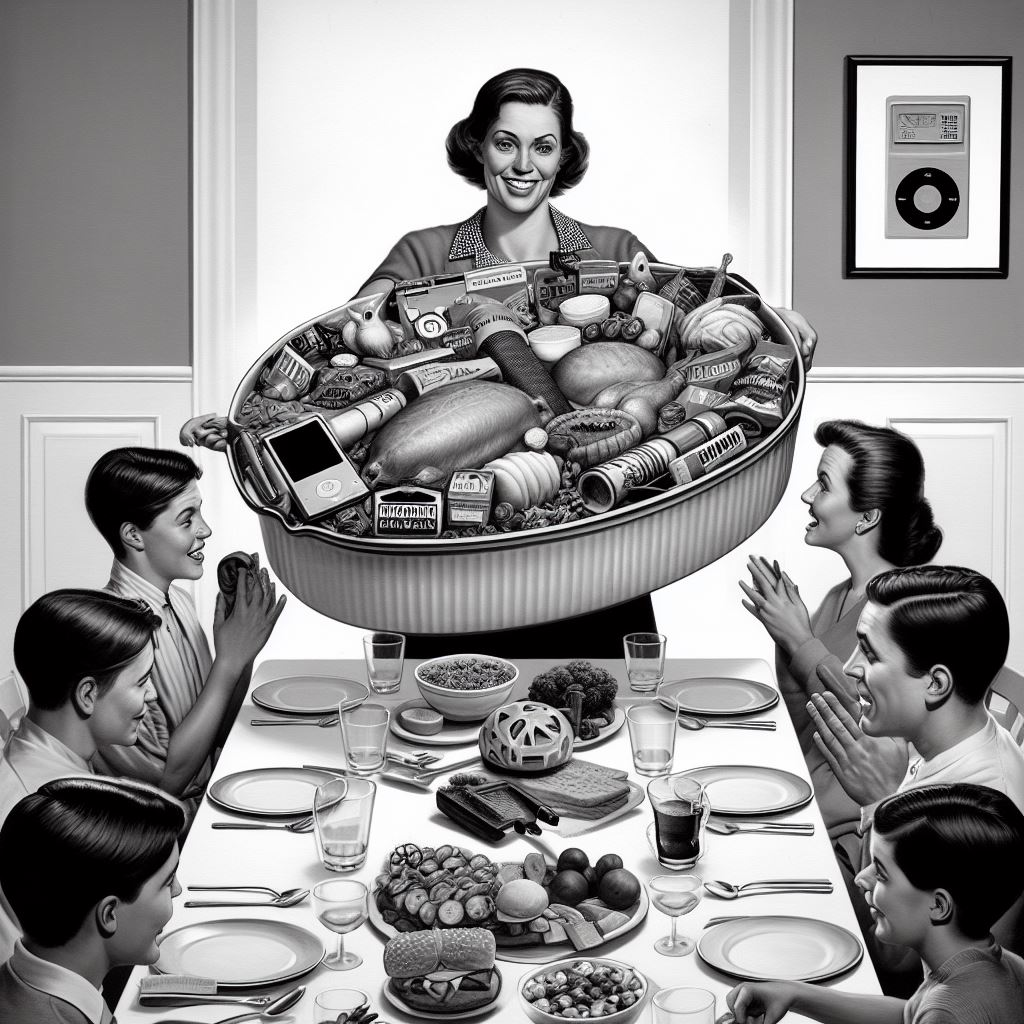
\includegraphics[scale=0.25]{./lecture_includes/wrong_covariates}
  \end{figure}
\end{frame}

\begin{frame}
  \begin{figure}
    
\includegraphics[scale=0.25]{./lecture_includes/dogs_unconfoundedness}
  \end{figure}
\end{frame}








\begin{frame}{Falsifications as a test}

\begin{itemize}
\item Covariates should not be affected by the treatment, so examining them as falsifications can help establish the credibility of unconfoundedness
\item Falsification exercises are sometimes versions of this -- a gun control law shouldn't affect automobile theft or petty larceny or average age of the state
\item Imbens and Rubin (2015) suggested using the lagged outcome (pre-treatment) as a way of checking, as those have similar confounder structures
\item But just be careful because without some understanding of the treatment assignment mechanism, you could make serious mistakes
\end{itemize}

\end{frame}

\begin{frame}
  \begin{figure}
    
\includegraphics[scale=0.25]{./lecture_includes/trail_runner}
  \end{figure}
\end{frame}

\begin{frame}
  \begin{figure}
    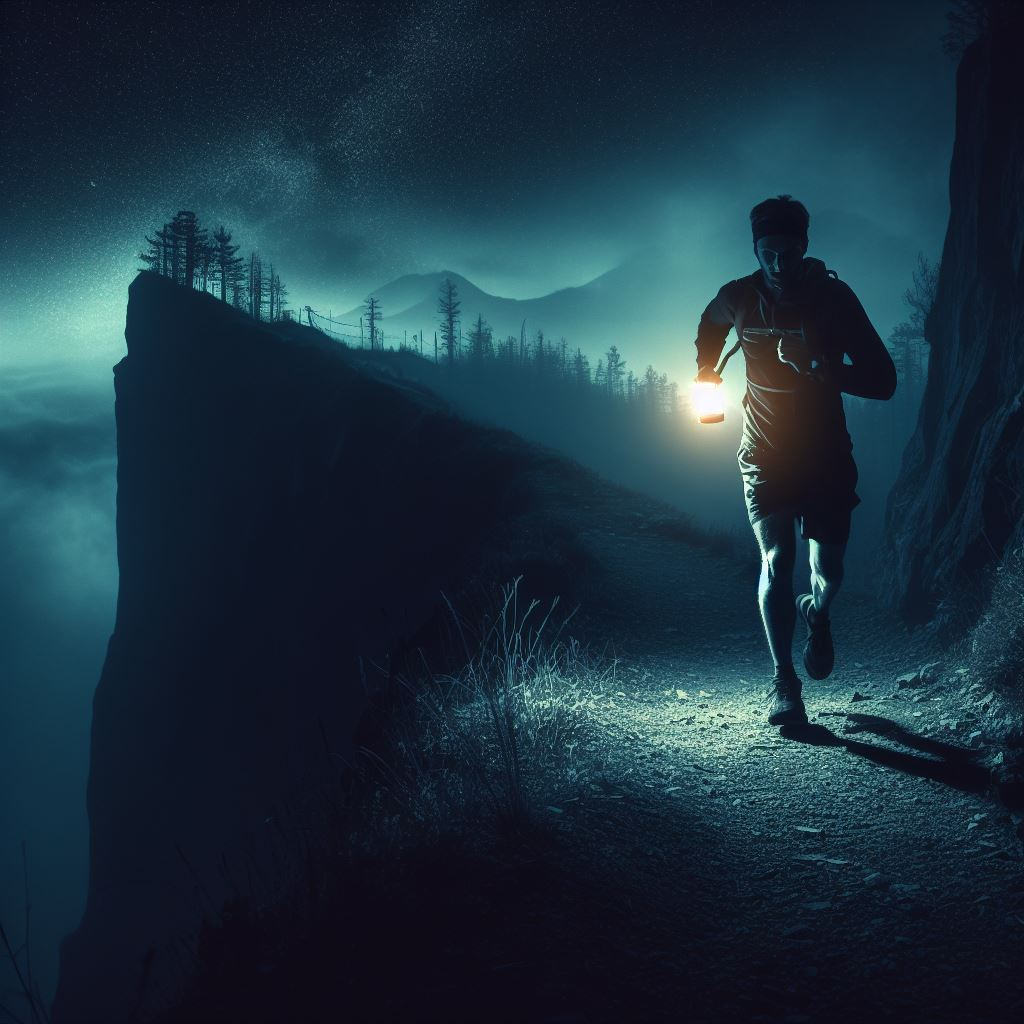
\includegraphics[scale=0.25]{./lecture_includes/trail_runner_2}
  \end{figure}
\end{frame}



\section{Unconfoundedness and Ignorable Treatment Assignment}

\subsection{Motivating estimation with an example}






\begin{frame}{Titanic example and a simple DAG}

\begin{itemize}

\item What if we wanted to know the causal effect of being seated in first class (D) on survival (Y) in the sinking of the Titanic cruiser in the early 20th century?  
\item Domain knowledge: as the Titanic sank, the captain called for women (W) and children (D) to go first

\end{itemize}

\end{frame}




\begin{frame}{Titanic DAG}

\begin{figure}
\begin{center}
\caption{Titanic sinking as a DAG}
\begin{tikzpicture}[node distance=2cm]
% nodes %
\node[text centered] (d) {$D$};
\node[below left of = d, text centered] (c) {$C$};
\node[above left of = d, text centered] (w) {$W$};
\node[right of = d, text centered] (y) {$Y$};
% edges %
\draw[->, line width= 1] (d) -- (y);
\draw[->, line width= 1] (c) -- (d);
\draw[->, line width= 1] (w) -- (d);
\draw[->, line width= 1] (c) -- (y);
\draw[->, line width= 1] (w) -- (y);
\end{tikzpicture}
\label{fig:backdoor_dag}
\end{center}
\end{figure}

\bigskip

Write down all paths, both direct from $D$ to $Y$ and indirect or ``backdoor paths'' 

\end{frame}



\begin{frame}{Simple DAG}

\begin{figure}
\begin{center}
\caption{A simple DAG illustrating selection on observables.}
\begin{tikzpicture}[node distance=2cm]
% nodes %
\node[text centered] (d) {$D$};
\node[below left of = d, text centered] (c) {$C$};
\node[above left of = d, text centered] (w) {$W$};
\node[right of = d, text centered] (y) {$Y$};
% edges %
\draw[->, line width= 1] (d) -- (y);
\draw[->, line width= 1] (c) -- (d);
\draw[->, line width= 1] (w) -- (d);
\draw[->, line width= 1] (c) -- (y);
\draw[->, line width= 1] (w) -- (y);
\end{tikzpicture}
\end{center}
\end{figure}

\bigskip

\begin{enumerate}
\item[1. ] $D\rightarrow Y$, the direct edge representing a causal effect with associated causal parameter like the ATE, ATT, etc. 
\end{enumerate}
\end{frame}



\begin{frame}{Simple DAG}

\begin{figure}
\begin{center}
\caption{The same simple DAG illustrating selection on observables only with the direct edge from $D$ to $Y$ deleted and backdoor $W$ blocked.}
\begin{tikzpicture}[node distance=2cm]
% nodes %
\node[text centered] (d) {$D$};
\node[below left of = d, text centered] (c) {$C$};
\node[above left of = d, text centered] (w) {$\mybox{W}$};
\node[right of = d, text centered] (y) {$Y$};
% edges %
\draw[->, line width= 1] (d) -- (y);
\draw[->, line width= 1] (c) -- (d);
\draw[->, line width= 1] (c) -- (y);
\end{tikzpicture}
\end{center}
\end{figure}

\bigskip

\begin{enumerate}
\item[2. ] $D\leftarrow \mybox{W} \rightarrow Y$ is a backdoor from $D$ to $Y$ through $W$. \textcolor{purple}{Block it}
\end{enumerate}
\end{frame}



\begin{frame}{Remaining variation after blocking}

\begin{figure}
\begin{center}
\caption{Visualization of Backdoor Criterion}
\begin{tikzpicture}[node distance=2cm]
% nodes %
\node[text centered] (d) {$D$};
\node[below left of = d, text centered] (c) {$\mybox{C}$};
\node[above left of = d, text centered] (w) {$\mybox{W}$};
\node[right of = d, text centered] (y) {$Y$};
% edges %
\draw[->, line width= 1] (d) -- (y);
\end{tikzpicture}
\end{center}
\end{figure}

\bigskip

\begin{enumerate}
\item[2. ] $D\leftarrow \mybox{W} \rightarrow Y$ is a backdoor from $D$ to $Y$ through $W$. \textcolor{purple}{Block it}
\item[3. ] $D\leftarrow \mybox{C} \rightarrow Y$ is a backdoor from $D$ to $Y$ through $C$. \textcolor{purple}{Block it}
\end{enumerate}
\end{frame}


\begin{frame}{Definition of Known and Quantified Confounders}
	
	
	\begin{block}{Definition of a Known and Quantified Confounder}
	Variable $C$ is a \emph{known} and \emph{quantified} \emph{confounders} if the researcher believes it causes units to select into treatment ($C \rightarrow D$) and also independently determine outcome $Y$, or $C \rightarrow Y$. Confounders are always known, which requires prior knowledge. And to be quantified, they must be correctly measured in your dataset.
	\end{block}
	
	
\end{frame}

\begin{frame}{Known and Quantified Confounder}

	\begin{itemize}
	\item Confounders may or may not be observed, but they must be known if they are confounders as confounders create backdoor paths from $D$ to $Y$
	\item Visually, solid lines means they are ``quantified'' (i.e., in the data), whereas dashed lines mean they are either not defined correctly or not in the dataset (``unobserved'')
	\item Backdoor criterion is appropriate only for known and quantified confounders -- if either known or quantified is missing, this material today is not to be used
	\end{itemize}

\end{frame}

\begin{frame}{DAG tells us what we need to condition on}

\begin{itemize}

\item If we ``block'' on $C$ and $W$, then the \emph{only} explanation of why $D$ and $Y$ are then correlated is causal
\item Depending on the model we estimate, and explicit assumptions made about potential outcomes, then we are able to identify an aggregate causal parameter
\item Let us now call $C$ and $W$ ``known and quantified confounders'' because the model said these were necessary, they were observed (no dashed line) and they were confounders
\item Let's add two more variables -- one we discussed already, but one we haven't

\end{itemize}

\end{frame}



\begin{frame}{Modification of the original DAG}

\begin{figure}
\begin{center}
\caption{A DAG illustrating confounders ($W$ and $C$) versus colliders ($B$) versus exogenous covariates $(X)$.}
\begin{tikzpicture}[node distance=2cm]
% nodes %
\node[text centered] (d) {$D$};
\node[below left of = d, text centered] (c) {$\mybox{C}$};
\node[above left of = d, text centered] (w) {$\mybox{W}$};
\node[above of = y, text centered] (x) {$X$};
\node[below of = y, text centered] (b) {$B$};
\node[right of = d, text centered] (y) {$Y$};
% edges %
\draw[->, line width= 1] (d) -- (y);
\draw[->, line width= 1] (d) -- (b);
\draw[->, line width= 1] (y) -- (b);
\draw[->, line width= 1] (x) -- (y);
\end{tikzpicture}
\label{fig:backdoor_dag}
\end{center}
\end{figure}

\begin{enumerate}
\item[4. ] Conditional on $C$ and $W$, the collider path $D \rightarrow B \leftarrow Y$ is closed by the collider $B$
\item[5. ] And $X$ never appears on any of our backdoor paths, so it is irrelevant, but it may be useful to include anyway
\end{enumerate}


\end{frame}




\begin{frame}{Covariate}
	
	
	\begin{block}{Definition of a Covariate}
	Variable $X$ is a covariate if it causes $Y$ but does not cause the treatment status $D$.
	\end{block}
	
	\begin{itemize}
	\item Think of it as explaining the outcome, but not correlated with the treatment variable (therefore it's in the error term of a regression model)
	\item Including $X$ in a model can increase precision of estimates of $D$ on $Y$ simply by reducing residual variance, but should have no effect on point estimates
	\item For us today, I am going to try to distinguish between ``confounders'' which are needed to estimate causal effects and ``covariates'' which help with precision 
	\end{itemize}
	
\end{frame}

\begin{frame}{Modification of the original DAG}

\begin{figure}
\begin{center}
\caption{A DAG illustrating confounders ($W$ and $C$) versus colliders ($B$) versus exogenous covariates $(X)$.}
\begin{tikzpicture}[node distance=2cm]
% nodes %
\node[text centered] (d) {$D$};
\node[below left of = d, text centered] (c) {$\mybox{C}$};
\node[above left of = d, text centered] (w) {$\mybox{W}$};
\node[above of = y, text centered] (x) {$X$};
\node[below of = y, text centered] (b) {$B$};
\node[right of = d, text centered] (y) {$Y$};
% edges %
\draw[->, line width= 1] (d) -- (y);
\draw[->, line width= 1] (d) -- (b);
\draw[->, line width= 1] (y) -- (b);
\draw[->, line width= 1] (x) -- (y);
\end{tikzpicture}
\label{fig:backdoor_dag}
\end{center}
\end{figure}

\begin{enumerate}
\item[5. ] You cannot get from $D$ to $Y$ via $B$ so it is a collider, but if you control for it, that path opens up and introduces selection bias (``bad controls'')
\end{enumerate}


\end{frame}

\begin{frame}{Two useful readings}

\begin{enumerate}
\item Cunningham (2023), ``Which variables do I need to control for?'' Substack post, \url{https://causalinf.substack.com/p/which-variables-do-i-need-to-control}
\item Cinelli, Forney, and Pearl (2022), ``A Crash Course in Good and Bad Controls'', forthcoming in \emph{Journal Sociological Methods and Research} (previously technical report R-493), available in our readings directory
\end{enumerate}

\end{frame}


\begin{frame}{}

  \begin{figure}
    
\includegraphics[scale=0.25]{./lecture_includes/scott_controls}
  \end{figure}

\end{frame}


\begin{frame}{}

  \begin{figure}
    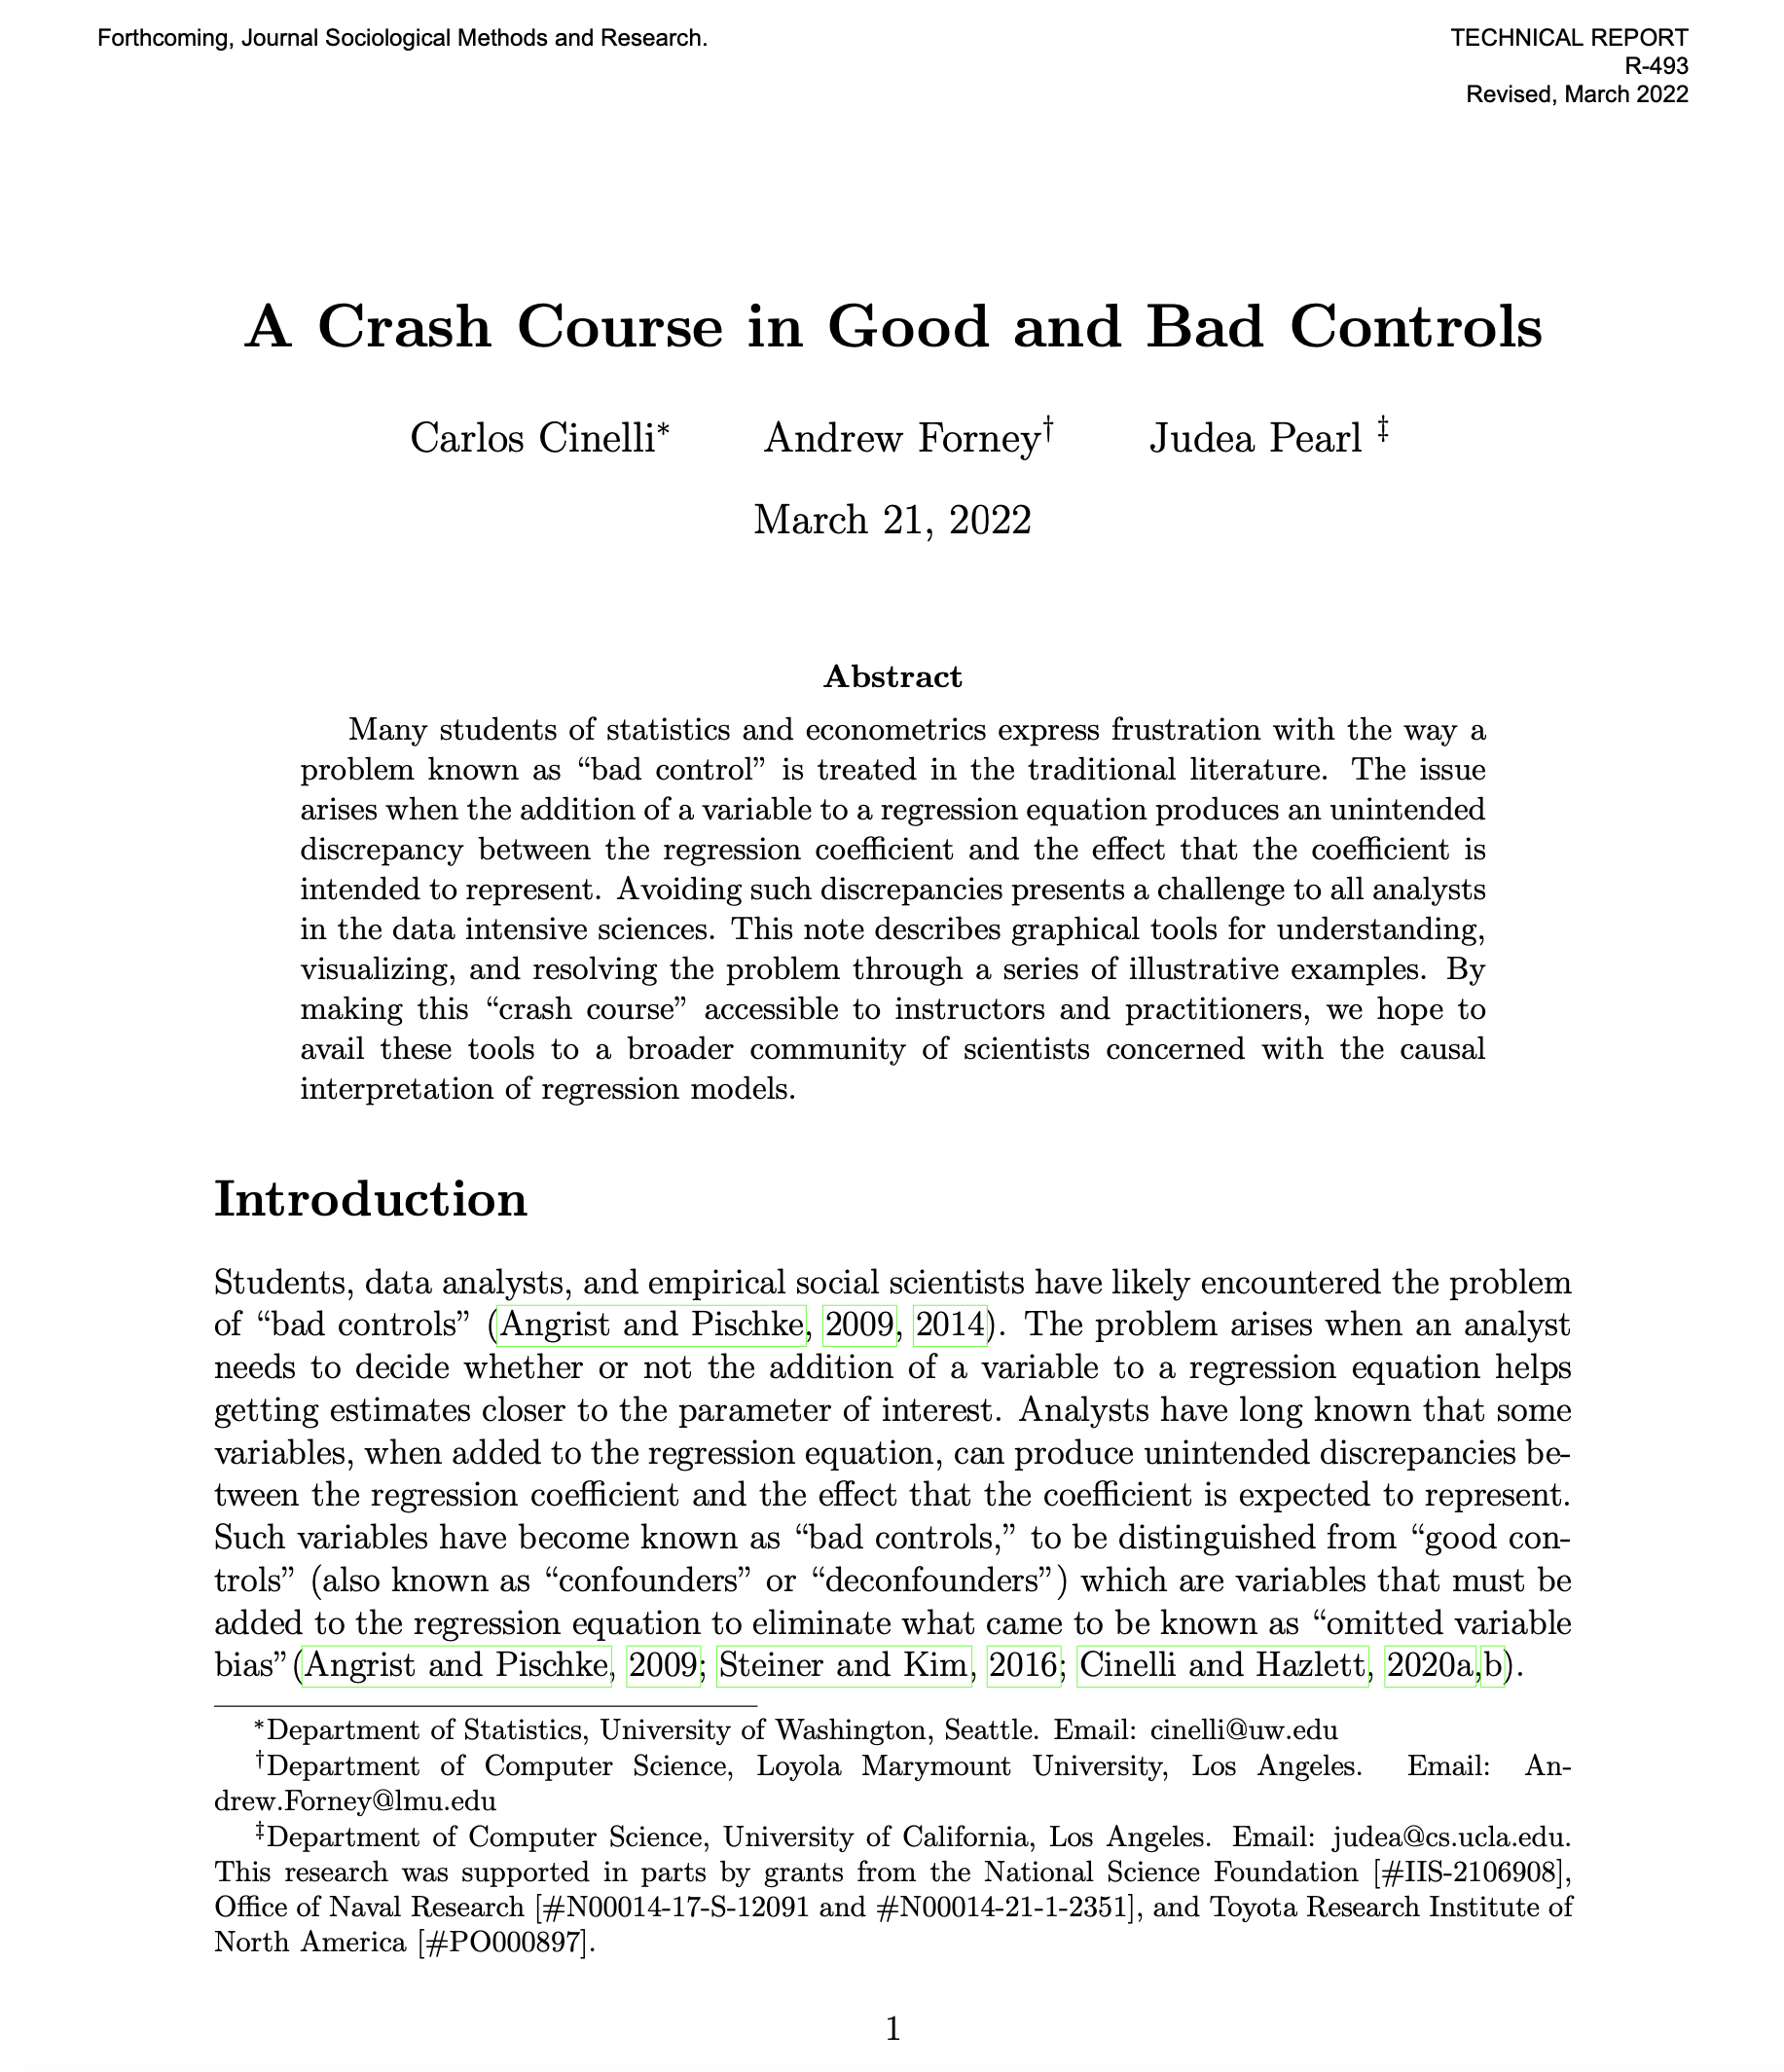
\includegraphics[scale=0.25]{./lecture_includes/crash_course}
  \end{figure}

\end{frame}





\subsection{Aggregate target parameters}


\begin{frame}{Defining the target parameter comes first}

\begin{itemize}
\item So you want to estimate causal effects using ``controls'' -- remember our steps, though -- step 1 is to define the parameter (e.g., $ATE$, $ATT$, $ATU$)
\item Also something called the $CATE$ -- conditional ATE which is an ATE for certain values of $X$ (e.g., ATE for men) -- which is quite common in ML because of the focus on estimating more targeted "individual treatment effects" defined by observables

\end{itemize}

\end{frame}

\begin{frame}{Defining the target parameter comes first}

\begin{itemize}
\item Covariate adjustment strategies like regression or matching can identify these, but they aren't the same in non-experimental data if there's heterogenous treatment effects (i.e., $\delta_i$ differs for different $i$ people)
\item So it is imperative up front you decide which aggregate causal parameter you're going to be trying to estimate as each one has different assumptions and different methodologies (as well as interpretations)

\end{itemize}

\end{frame}




\subsection{Assumptions}


\begin{frame}{Aggregate causal parameters have missing potential outcomes}


\begin{itemize}
\item Every aggregate causal parameter is missing some potential outcome (e.g., ATT is missing $E[Y^0|D=1])$
\item If we are going to estimate the ATT, then it must be we are estimating $E[Y^0|D=1]$ somehow, but how?
\item If we are using controls, then we in some way, shape or form ``filling in'' the missing counterfactual using the covariates of the comparison group
\item ``At some level, all methods for causal inference can be viewed as imputation methods, although some more explicitly than others.'' -- Imbens and Rubin (2015)

\end{itemize}


\end{frame}


\begin{frame}{Assumptions}

\begin{itemize}

\item When attempting to estimate aggregate causal parameters using covariate adjustment, there are two assumptions

	\begin{enumerate}
	\item \textbf{Unconfoundedness}:  fairly controversial to some because of what it implies about human behavior
	\item \textbf{Common support}: since most people stop at assumption 1, there's much less attention to common support
	\end{enumerate}
\item Today we will assume you satisfy unconfoundedness, but because we are solely focused on DML, I will be mostly moving around common support to go directly into regression based methods
\end{itemize}

\end{frame}


\begin{frame}[plain]

	\begin{block}{Identifying assumption I: Unconfoundedness}
	$(Y_i^0$, $Y_i^1)$ $\independent{D} | X_i$. There exists a set $X$ of known and quantified confounders such that after adjusting for them, treatment assignment is \emph{independent of potential outcomes}.
	\end{block}
	
	\begin{itemize}
	\item Conditional on $X$, treatment assignment is randomly distributed (i.e., independent of both potential outcomes) -- strong assumption
	\item For a large group of people within the same strata of $X$, this assumption states they choose treatments by flipping coins (not because they think the treatment helped them)
	\item Eliminating all backdoor paths on a DAG through blocking satisfies unconfoundedness; also called ignorability
	\end{itemize}
\end{frame}


\begin{frame}[plain]

	\begin{block}{Identifying assumption I: Unconfoundedness}
	$(Y_i^0$, $Y_i^1)$ $\independent{D} | X_i$. There exists a set $X$ of known and quantified confounders such that after adjusting for them, treatment assignment is \emph{independent of potential outcomes}.
	\end{block}
	
	\begin{eqnarray*}
	\alert{E[Y^0 | D=1, X=x]} &=& E[Y^0 | D=0, X=x] \\
	E[Y^1 | D=1, X=x] &=& \alert{E[Y^1 | D=0, X=x] }
	\end{eqnarray*}
	
Unconfoundedness justifies substituting units in treatment for control based on $X=x$ -- but only if there are exact matches
	
	
\end{frame}

\begin{frame}{Economic meaning of backdoor criterion}

\begin{itemize}
\item When people choose their own treatments, attempting to estimate aggregate causal parameters using covariates that conditional on those covariates, they are \emph{randomizing choices}
\item See my substack post, ``Why do economists so dislike `conditional independence''? (January 4, 2023) at \url{https://causalinf.substack.com/p/why-do-economists-so-dislike-conditional}
\end{itemize}

\end{frame}

\begin{frame}{}

  \begin{figure}
    
\includegraphics[scale=0.25]{./lecture_includes/disliking_controls}
  \end{figure}

\end{frame}







\begin{frame}[plain]

	\begin{block}{Identifying assumption II: Common support}
	For ranges of $X$, there is a positive probability of being both treated and untreated
	\end{block}
	
	\begin{itemize}
	\item There exists units in treatment and control with same values of $X$ -- you can't make the substitutions otherwise
	\item Dimension $k$ means every specific combination of the conditioning set (e.g., not males and old, but adult males, adult females, youth male, youth female)
	\item Testable because common support is observable unlike unconfoundedness, but as you can imagine if the dimensions of $X$ gets large (and with a continuous covariate it's infinite!) then it won't hold in any finite sample!
	\end{itemize}
	
	
\end{frame}



\begin{frame}{Assumptions combined}
	
But if we have them both (represented below), we can even outside of an RCT estimate the ATE through nonparametric matching
  \begin{enumerate}
		\item $(Y^1,Y^0) \independent{D} | X$ (strong unconfoundedness)
		\item $0<Pr(D=1|X)<1$ with probability one (common support)
  \end{enumerate}

\bigskip
Comparing groups of individuals \emph{who have the same values of} $X$, treatment is no longer based gains, $\delta$. 

\bigskip

The second term implies we have people in treatment and control for every strata of $X$
\end{frame}


\begin{frame}{Estimating ATE with Assumptions}


	\begin{itemize}
	\item Unconfoundedness lets you use $Y^0_j$ from control group as $i$'s $\alert{Y^0_i}$ and $Y^1_i$ from treatment group as $j$'s $\alert{Y^1_j}$ using $X$ as the matching guide
		\begin{eqnarray*}
		E[Y^1-Y^0|X] &=& E[Y^1 - Y^0 | X,D=1] \\
		&=&E[Y|X,D=1] - E[Y|X,D=0]
		\end{eqnarray*}
	\item Common support (Assumption 2) allows the match to take place as well as weight over the covariate distribution
		\begin{eqnarray*}
		\delta_{ATE} &=&E[Y^1-Y^0] = E\bigg[ E[Y^1 - Y^0 \ \vert \ X] \bigg] \\
		&=& \int E[Y^1 - Y^0 |X,D=1] dPr(X) \\
		&=& \int \left(E[Y|X,D=1] - E[Y|X,D=0]\right)dPr(X)
		\end{eqnarray*}
	\end{itemize}

\end{frame}



\begin{frame}{Maybe You Want the ATT}

ATE requires conditional independence with respect to both $Y^1$ and $Y^0$ which would mean complete irrationality imo (I seem to be alone in describing strong unconfoundedness this way)

\bigskip

But maybe you actually want the ATT, we can go with strictly weaker assumptions -- weak unconfoundedness and weak overlap -- and therefore slightly more rationality

\bigskip

You can get a PhD because you care about your happiness with one $Y^1$; you just have to have acted independent of what you gave up $Y^0$

\end{frame}

\begin{frame}{Maybe You Want the ATT}

\begin{itemize}
\item ATE -- it's the summarizing of all treatment effects at the unit level. So think of it as a population parameter and if you are confused, ask yourself ``Do I want to know the causal effect for every possible person?''
\item ATT -- it's summarizing the treatment effects only for the treatment group.  Think of it as a subpopulation parameter.  Do you want to know the causal effect but only for the treatment group?
\item Efficacy of vaccines (ATE) versus efficacy of ventilators (ATT)
\item Popularity of DiD and synth suggest that the ATT is a desirable parameter as they only identify the ATT, not the ATE, under parallel trends
\end{itemize}

\end{frame}



\begin{frame}{ATT Identification}

We can modify those assumptions and weaken both which helps a lot

\begin{enumerate}
  \item $Y^0 \independent{D} | X$ (weak unconfoundedness)
  \item $Pr(D=1|X)<1$ (with $Pr(D=1)>0$) (weak support)
\end{enumerate}

\bigskip

We don't need full common support because we don't need to find counterfactuals for the control group -- we only need units in the control group that match with our treatment group

\bigskip

Selection is weaker too, like I said -- they are not entirely irrational, but who knows if it helps you

\end{frame}



\begin{frame}{Estimating ATT}


Weighted averages under both assumptions:
		\begin{eqnarray*}
		\delta_{ATT} &=& \int \left(E[Y|X,D=1] - E[Y|X,D=0]\right)dPr(X|D=1)
		\end{eqnarray*}
We match units in treatment and control because under weak unconfoundedness they're substitutable, and we use weak common support so that we can actually do it, then we take weighted averages over the differences.  

\bigskip

You could also flip out independence with respect to $Y^1$ and discuss common support for the control group and get back to the ATU too
	
\end{frame}



\begin{frame}{Estimators}

\begin{itemize}

\item Now we will explore estimators that for lack of a better word ``use covariates'' to estimate aggregate causal parameters
\item I will be bundling them around a few topics: exact matching, inexact matching, and regressions
\item Themes about heterogeneous treatment effects, common support and correct (and incorrect) regression specifications will be common

\end{itemize}

\end{frame}





\section{Estimators}

\subsection{Subclassification}

\begin{frame}
\begin{itemize}

\item Multivariate regression goes back to Yule (19th century)
\item Weighting goes back to Cochran (late 60s)
\item Matching seems to be from the 1970s
\item Novel insights about regression methods are based on Oaxaca-Blinder in the 1970s, and more recently Kline and Wooldridge
\item DML as we said is Chernozhukov, et al. (2016) 
\end{itemize}

\end{frame}


\begin{frame}{Subclassification method}

\begin{itemize}

\item Wanting to show subclassification as an early effort to tackle covariates, but which ultimately cannot handle large features due to common support issues before moving into regression then DML
\item Titanic sank on maiden voyage April 15, 1912 after hitting an iceberg in North Atlantic
\item 2200 on board, but only 700 survived, despite 20 lifeboats with 60 capacity (1200 potential lives could've been saved)
\item Women and children first was a maritime rule to ration lifeboats, but there were different cabins (1st class, 2nd class, etc.) on different levels with different proximity to boats
\item What was the causal effect of 1st class on survival adjusting for $W$ and $C$?
\end{itemize}

\end{frame}


\begin{frame}{Exercise: Titanic DAG}

\begin{figure}
\begin{center}
\caption{Women $W$ and children $C$ first maritime rule is a confounder for estimating first class $D$ effect on surviving $Y$}
\begin{tikzpicture}[node distance=2cm]
% nodes %
\node[text centered] (d) {$D$};
\node[below left of = d, text centered] (c) {$\mybox{C}$};
\node[above left of = d, text centered] (w) {$\mybox{W}$};
\node[right of = d, text centered] (y) {$Y$};
% edges %
\draw[->, line width= 1] (d) -- (y);
\draw[->, line width= 1] (c) -- (d);
\draw[->, line width= 1] (w) -- (d);
\draw[->, line width= 1] (c) -- (y);
\draw[->, line width= 1] (w) -- (y);
\end{tikzpicture}
\label{fig:titanic}
\end{center}
\end{figure}

\bigskip

Backdoor criterion can be satisfied by blocking on $W$ and $C$.  These are our known confounders.  Now we just need data to see if it's quantified.

\end{frame}

\begin{frame}{Titanic exercise}

\begin{enumerate}
\item \textbf{Stratify the confounders}: Our age and sex variables are both binary, so we can only create four strata: male children, female children, male adults, female adults
\item \textbf{Calculate differences within strata}: Calculate average survival rates for each group within each of the four strata and difference within strata
\item \textbf{Calculate probability weights}: Count the number of people in each strata and divide by the total number of souls aboard (crew and passengers)
\item \textbf{Aggregate differences across strata using weights}: Estimate the ATE by aggregating the difference in survival rates over the four strata with each strata-specific difference weighted by that strata's weight
\end{enumerate}


\end{frame}

\begin{frame}{Table 1: Standard balance table}

{\renewcommand{\arraystretch}{1.1}
\tabcolsep=1.3\tabcolsep 		
\begin{table}\small\index{rolling!3}
\caption{Differences in female and adult passengers by first class status on the Titanic. }
\centering
\begin{tabular}{lcc|cc}
\toprule
\multicolumn{1}{c}{\textbf{Variable name}}&
\multicolumn{2}{c}{\textbf{First class}}&
\multicolumn{2}{c}{\textbf{All other classes}}\\
\multicolumn{1}{c}{}&
\multicolumn{1}{c}{Obs}&
\multicolumn{1}{c}{Mean}&
\multicolumn{1}{c}{Obs}&
\multicolumn{1}{c}{Mean}\\
\midrule
Percent adult		&	325 	& 98.2\% & 1,876 & 94.5\% \\
Percent female		& 	325	& 44.6\% & 1,876 & 17.3\% \\
\bottomrule
\end{tabular}
\label{tab:titanic-age}
\end{table}}
\end{frame}


\begin{frame}{Table 2: Stratified sample}

{\renewcommand{\arraystretch}{1.1}
\tabcolsep=1.3\tabcolsep 		
\begin{table}\small\index{rolling!3}
\caption{Counts and Titanic survival rates by strata and first class status.}
\centering
\begin{tabular}{lcc|cc|c}
\toprule
\multicolumn{1}{c}{\textbf{}}&
\multicolumn{2}{c}{\textbf{First class}}&
\multicolumn{2}{c}{\textbf{All other classes}}&
\multicolumn{1}{c}{\textbf{}}\\
\multicolumn{1}{l}{Strata}&
\multicolumn{1}{c}{Obs}&
\multicolumn{1}{c}{Mean}&
\multicolumn{1}{c}{Obs}&
\multicolumn{1}{c}{Mean}&
\multicolumn{1}{c}{Total}\\
\midrule
Male adult		& 175	& 0.326	& 1,492	& 0.188	& 1,667 \\
Female adult	& 144	& 0.972	& 281	& 0.626	& 425 \\
Male child		& 5		& 1		& 59		& 0.407 	& 64\\
Female child	& 1		& 1		& 44		& 0.613 	& 45\\
\midrule
Total	observations	& 325	&&	1,876	 && 2,201\\
\bottomrule
\end{tabular}
\label{tab:titanic-counts}
\end{table}}


\end{frame}

\begin{frame}{Table 3: Estimates of aggregate parameter}

{\renewcommand{\arraystretch}{1.1}
\tabcolsep=1.3\tabcolsep 		
\begin{table}\tiny\index{rolling!3}
\caption{Differences in survival rates, stratification weights, and estimates of parameters}
\centering
\begin{tabular}{lc|ccc}
\toprule
\multicolumn{1}{l}{\textbf{Strata}}&
\multicolumn{1}{c}{\textbf{Differences in Survival Rates}}&
\multicolumn{1}{c}{\textbf{Weight$_{k,ATE}$}}&
\multicolumn{1}{c}{\textbf{Weight$_{k,ATT}$}}&
\multicolumn{1}{c}{\textbf{Weight$_{k,ATU}$}}\\
\midrule
Male adult		& 0.138 &	0.76 &	0.54	&0.80	\\
Female adult	& 0.346 &	0.19 &	0.44	&0.15	\\
Male child		& 0.593 &	0.03 &	0.02	&0.03	\\
Female child	& 0.387 &	0.02 &	0.00	&0.02	\\
\midrule
\multicolumn{1}{l}{\textbf{}}&
\multicolumn{1}{c}{\textbf{No stratification}}&
\multicolumn{3}{c}{\textbf{Stratification weighted estimates}}\\

 & $\widehat{\textbf{SDO}}$& $\widehat{\textbf{ATE}}$ & $\widehat{\textbf{ATT}}$ & $\widehat{\textbf{ATU}}$ \\
\midrule
\textbf{Estimated coefficient}& 0.35 & 0.20 & 	0.24	 & 0.19   \\
\bottomrule
\end{tabular}
\label{tab:titanic-weights}
\end{table}}

\end{frame}

\begin{frame}{Drop the one female child}

\begin{itemize}
\item We were able to estimate all three causal effect parameters because for all four strata there were units in both treatment and control
\item But if we dropped the only female child in first class from the data, we'd be in trouble bc there wouldn't be any way to calculate a difference for that group
\item But what could we identify?

\end{itemize}

\end{frame}

\begin{frame}

\begin{table}\small\index{rolling!3}
\caption{Counts and Titanic survival rates by strata and first class status.}
\centering
\begin{tabular}{lcc|cc|c}
\toprule
\multicolumn{1}{c}{\textbf{}}&
\multicolumn{2}{c}{\textbf{First class}}&
\multicolumn{2}{c}{\textbf{All other classes}}&
\multicolumn{1}{c}{\textbf{}}\\
\multicolumn{1}{l}{Strata}&
\multicolumn{1}{c}{Obs}&
\multicolumn{1}{c}{Mean}&
\multicolumn{1}{c}{Obs}&
\multicolumn{1}{c}{Mean}&
\multicolumn{1}{c}{Total}\\
\midrule
Male adult		& 175	& 0.326	& 1,492	& 0.188	& 1,667 \\
Female adult	& 144	& 0.972	& 281	& 0.626	& 425 \\
Male child		& 5		& 1		& 59		& 0.407 	& 64\\
Female child	& 0		& n/a		& 44		& 0.613 	& 44\\
\midrule
Total	observations	& 324	&&	1,876	 && 2,200\\
\bottomrule
\end{tabular}
\label{tab:titanic-counts2}
\end{table}

\end{frame}

\begin{frame}{ATT is the only one we can get}

\begin{eqnarray}
\widehat{\delta}_{ATT} &=& (0.137 \times 0.54) + (0.346 \times 0.44) + (0.593 \times 0.02)  \nonumber \\
&=& 0.24\text{ or 24 percentage points}
\end{eqnarray}

\end{frame}

\begin{frame}

\begin{table}\tiny\index{rolling!3}
\caption{Differences in survival rates, stratification weights, and estimates of parameters without perfect stratification}
\centering
\begin{threeparttable}
\begin{tabular}{lc|ccc}
\toprule
\multicolumn{1}{l}{\textbf{Strata}}&
\multicolumn{1}{c}{\textbf{Differences in Survival Rates}}&
\multicolumn{1}{c}{\textbf{Weight$_{k,ATE}$}}&
\multicolumn{1}{c}{\textbf{Weight$_{k,ATT}$}}&
\multicolumn{1}{c}{\textbf{Weight$_{k,ATU}$}}\\
\midrule
Male adult		& 0.137 	&	0.76 &	0.54	&0.80	\\
Female adult	& 0.346 	&	0.19 &	0.44	&0.15	\\
Male child		& 0.593 	&	0.03 &	0.02	&0.03	\\
Female child	& n/a 	&	n/a 	&	n/a	&0.02	\\
\midrule
\multicolumn{1}{l}{\textbf{}}&
\multicolumn{1}{c}{\textbf{No stratification}}&
\multicolumn{3}{c}{\textbf{Stratification weighted estimates}}\\

 & $\widehat{\textbf{SDO}}$& $\widehat{\textbf{ATE}}$ & $\widehat{\textbf{ATT}}$ & $\widehat{\textbf{ATU}}$ \\
\midrule
\textbf{Estimated coefficient}& 0.35 & n/a & 	0.24	 & n/a  \\
\bottomrule
\end{tabular}
\begin{tablenotes}
\tiny
\item 
Differences in survival rates, stratification weights, and estimated parameters. All coefficients should be multiplied by 100 to get a percentage point change in survival rate as a result of having a first class cabin. Note that the SDO is a simple difference in mean outcomes and therefore \emph{not} a weighted average over the strata differences.  But the estimated ATE, ATT and ATU parameters are weighted averages in difference in means using corresponding stratification weights. 
\end{tablenotes}
\end{threeparttable}
\label{tab:titanic-weights2}
\end{table}


\end{frame}

\begin{frame}{Why did this happen?}

\begin{itemize}

\item Stratification requires having units in both groups for every value of $X$ to get ATE
\item If you want the ATT, you have to have units in the control group for every treated group based on its value of $X$ (female children weren't treated, so didn't matter)
\item If you want the ATU, you have to have units in the treatment group for every treated group based on its value of $X$ (female children weren't treated, so did matter)
\item This has a technical word we are going to learn more about called a ``lack of common support''
\end{itemize}

\end{frame}

\begin{frame}{Curse of Dimensionality}
	
	\begin{itemize}
	\item Stratification methods break down in finite samples because as increase the number of covariates, the "dimension" grows even faster -- dimensions and covariates aren't the same in other words
	\item Assume we have $k$ covariates and we divide each into 3 coarse categories (e.g., age: young, middle age, old; income: low, medium, high, etc.)
	\item The number of strata is $3^k$. For $k=10$, then it's $3^{10}=59,049$
	\item The curse of dimensionality is based on the slices of all interactions of the covariates, not just the covariates, and that explodes fast
	\end{itemize}
\end{frame}

\begin{frame}{Empty cells}
	
	\begin{itemize}
	\item When some slice is empty, it means there's no one in that cell -- so maybe you don't have any female children in first class, but you do have them in other cabins
	\item When you have empty cells, you can't match within that dimension of the data, and so the "curse of dimensionality" is one of the reasons why the kitchen sink approach breaks down so fast
	\item Matching methods really force us to see these curses; they're often hidden from OLS because OLS (as we'll see) overcomes the problem by just assuming a linearity (it doesn't match; it extrapolates)
	\end{itemize}
\end{frame}	



\subsection{Regression}

\begin{frame}{Moving into regression}

\begin{itemize}

\item If we have unconfoundedness and common support -- complete common support -- then an unbiased estimate of these aggregate causal parameters is possible using nonparametric matching
\item But when we have a large number of covariates, we do not have common support because of the curse of dimensionality, and regression tends to be used instead (and therefore ML too)
\item Let's look at a proof by Imbens and Rubin explaining the additional assumptions needed by regression generally

\end{itemize}

\end{frame}

\begin{frame}{Core OLS assumptions}

\begin{itemize}
\item Return to OLS model with additive covariates  controls: $$Y_i = \alpha + \delta D_i + \beta X_i + \gamma Z_i + \varepsilon_i$$
\item Which average treatment effect parameter does $\widehat{\delta}$ estimate?  What assumptions are imposed by exogeneity?
\item This hopefully is where I'll be able to convince you of how important it is that you identify ahead of time \emph{which} causal effect
\item This is \textbf{not} a criticism of OLS but rather of that specification above
\end{itemize}

\end{frame}

\begin{frame}{OLS Assumptions}

\begin{itemize}

\item Typically we assume that the mean error is zero conditional on all covariates, called exogeneity
\item This is a pregnant assumption as it turns out
\item Imbens and Rubin discussed it in their book on causal inference from 2015
\item I'll pull out their quote and proof but we will then discuss some other materials

\end{itemize}

\end{frame}


\begin{frame}{OLS Assumptions}

	\begin{quote} 
	``In many empirical studies in social sciences, causal effects are estimated through linear regression, where, typically it is implicitly assumed that in the super-population, $$E[Y_i^D | X_i] = \alpha + \delta_{sp} \cdot D + X_i \beta$$ for some values of the three unknown parameters, $\alpha$, $\delta_{sp}$ and $\beta$ where $\delta_{sp} = E_{sp} [ Y_i^1 - Y_i^0]$.''
	\end{quote}
	
\end{frame}

\begin{frame}{What about OLS?  (Imbens and Rubin 2015)}

\begin{quote}
``Defining $\varepsilon_i = Y_i - \delta_{sp} \cdot D_i - X_i \beta$ so that we can write $$Y_i = \alpha + \delta_{sp} \cdot D_i + X_i \beta  + \varepsilon_i$$ it is then assumed that $$\varepsilon_i \independent D_i, X_i$$This assumption is often referred to as \textbf{exogeneity} of the treatment (and the pre-treatment variables) in the econometrics literature.''

\end{quote}

\end{frame}

\begin{frame}{OLS Assumptions}

\begin{quote}
``The regression function is interpreted as a causal relation, in our sense of the term ``causal'', namely that if we manipulate the treatment $D_i$, then tht outcome would change in expectation by an amount $\delta_{sp}$.  Hence in the potential outcomes formulation, we have 
\begin{eqnarray*}
Y_i^0 &=& \alpha + X_i \beta + \varepsilon_i \\ 
Y_i^1 &=& Y_i^0 + \delta_{sp}
\end{eqnarray*} 

\end{quote}
	
\end{frame}

\begin{frame}{OLS Assumptions}

\begin{quote}
``Then, because $\varepsilon_i$ is a function of $Y^0_i$ and $X_i$ given the parameters, $$Pr(D_i=1 | Y_i^0, Y_i^1 X_i ) = Pr(D_i | \varepsilon_i, X_i),$$ and by exogeneity of the treatment indicator, we have $$Pr(D_i|\varepsilon_i, X_i) = Pr(D_i | X_i)$$ and thus [conditional independence] holds.'' 
\end{quote}

\end{frame}

\begin{frame}{OLS Assumptions}

\begin{quote}
``However, the exogeneity assumption combines unconfoundedness with functional form and constant treatment effect assumptions that are quite strong, and arguably unnecessary.'' -- Imbens and Rubin (2015)
\end{quote}

\end{frame}

\begin{frame}{Great quote}

\begin{quote}
``OLS is \dots the linear projection of Y on D and X [and] provides the best linear predictor of Y given D and X (Angrist and Pishcke 2009).  However, if our goal is to conduct causal inference, then this is not, in fact, a good reason to use this method.  OLS is `best' in predicting actual outcomes, but causal inference is about predicting [fictional potential] outcomes.  \dots In other words, OLS \dots is optimal for predicting `what is'.  Instead we are interested in predicting `what would be' if treatment were assigned differently.'' - Tymon Sloczynski, Restat 2022
\end{quote}

\end{frame}




\begin{frame}{Prediction vs causal inference and OLS}




\begin{itemize}
\item OLS is the ``best linear predictor'' given the covariates because it minimizes the sum of all the residuals (squared)
\item So it's like it finds a \emph{line} that goes through the data in such a way that the prediction error is on average as small as possible
\item But out of sample is another matter -- that line \emph{fits the data} and ML has been about trying to improve it for prediction \emph{out of the data}
\item But to Tymon's point, that still isn't causal inference because in causal inference we are predicting fictional counterfactuals, not realized outcomes

\end{itemize}

\end{frame}




\begin{frame}{Constant Treatment Effects and Linearity}

Most commonly used method is OLS where the outcome is an additive model of the observed outcome, $Y$, on the treatment, $D$, and covariates, $X$ like:

\begin{eqnarray*}
Y_{i} &=& \alpha + \delta D_i + \beta_1 X_i +  \varepsilon_i \\
\end{eqnarray*}

Take conditional expectations 

\begin{eqnarray*}
E[Y_i | D_i = 1, X_i] &=& \alpha + \delta E[D_i | D_i=1, X_i] + \beta_1 E[X_i | D_i=1, X_i] \\
E[Y_i | D_i = 0, X_i] &=& \alpha + \delta E[D_i | D_i=0, X_i] + \beta_1 E[X_i | D_i=0, X_i] 
\end{eqnarray*}

\end{frame}

\begin{frame}{Constant Treatment Effects and Linearity}

Replace realized variables with potential notation (both outcomes and covariates):
\begin{eqnarray*}
E[Y^1_i | D_i = 1,X_i] &=& \alpha + \delta + \beta_{11} E[X^1_i | D_i=1, X_i] \\
E[Y^0_i | D_i = 0,X_i] &=& \alpha + \beta_{01} E[X^0_i | D_i=0, X_i] 
\end{eqnarray*}

\bigskip

$X^1$ is the effect of $X$ on $Y^1$ when treated and $X^0$ is effect on $Y^0$ when not treated; note if treatment changes $X$ then $X^1 \neq X^0$ and it will be a problem


\end{frame}


\begin{frame}{Constant Treatment Effects and Linearity}

With a binary treatment variable, the OLS estimator is equivalent to simple difference in conditional means:

\begin{eqnarray*}
\widehat{\delta} &=& E[Y^1_i | D_i = 1, X_i]  - E[Y^0_i | D_i = 0, X_i]  \\
 &=& \bigg (\alpha + \delta E[D_i | D_i=1, X_i] + \beta_{11} E[X^1_i | D_i=1, X_i] \bigg ) \\
&& - \bigg (\alpha + \delta E[D_i | D_i = 0, X_i] + \beta_{01} E[X^0_i | D_i = 0, X_i] \bigg ) \\
&=& \delta + \beta_{11} E[X^1_i | D_i =1, X_i] - \beta_{01} E[X^0_i | D_i = 0, X_i] 
\end{eqnarray*}

\bigskip

OLS model requires: (1) linearity, (2)  treatment cannot change covariate values (e.g., bad controls), (3) $\beta_{11}=\beta_{01}$ (homogenous treatment effects with respect to $X$).  

\end{frame}

\begin{frame}{Simulation}

\begin{itemize}

\item Simulation will have linear DGP, heterogeneity with respect to covariates and common support violation (1000 trials)
\item Will show a variety of estimators and specifications so that we see how to recover causal parameters with regression and matching
\item Focus is on estimated ATE and estimated ATT under a variety of specifications
\end{itemize}

\end{frame}

\begin{frame}{Heterogenous Treatment Effects wrt $X$}

\begin{figure}[!t]\centering
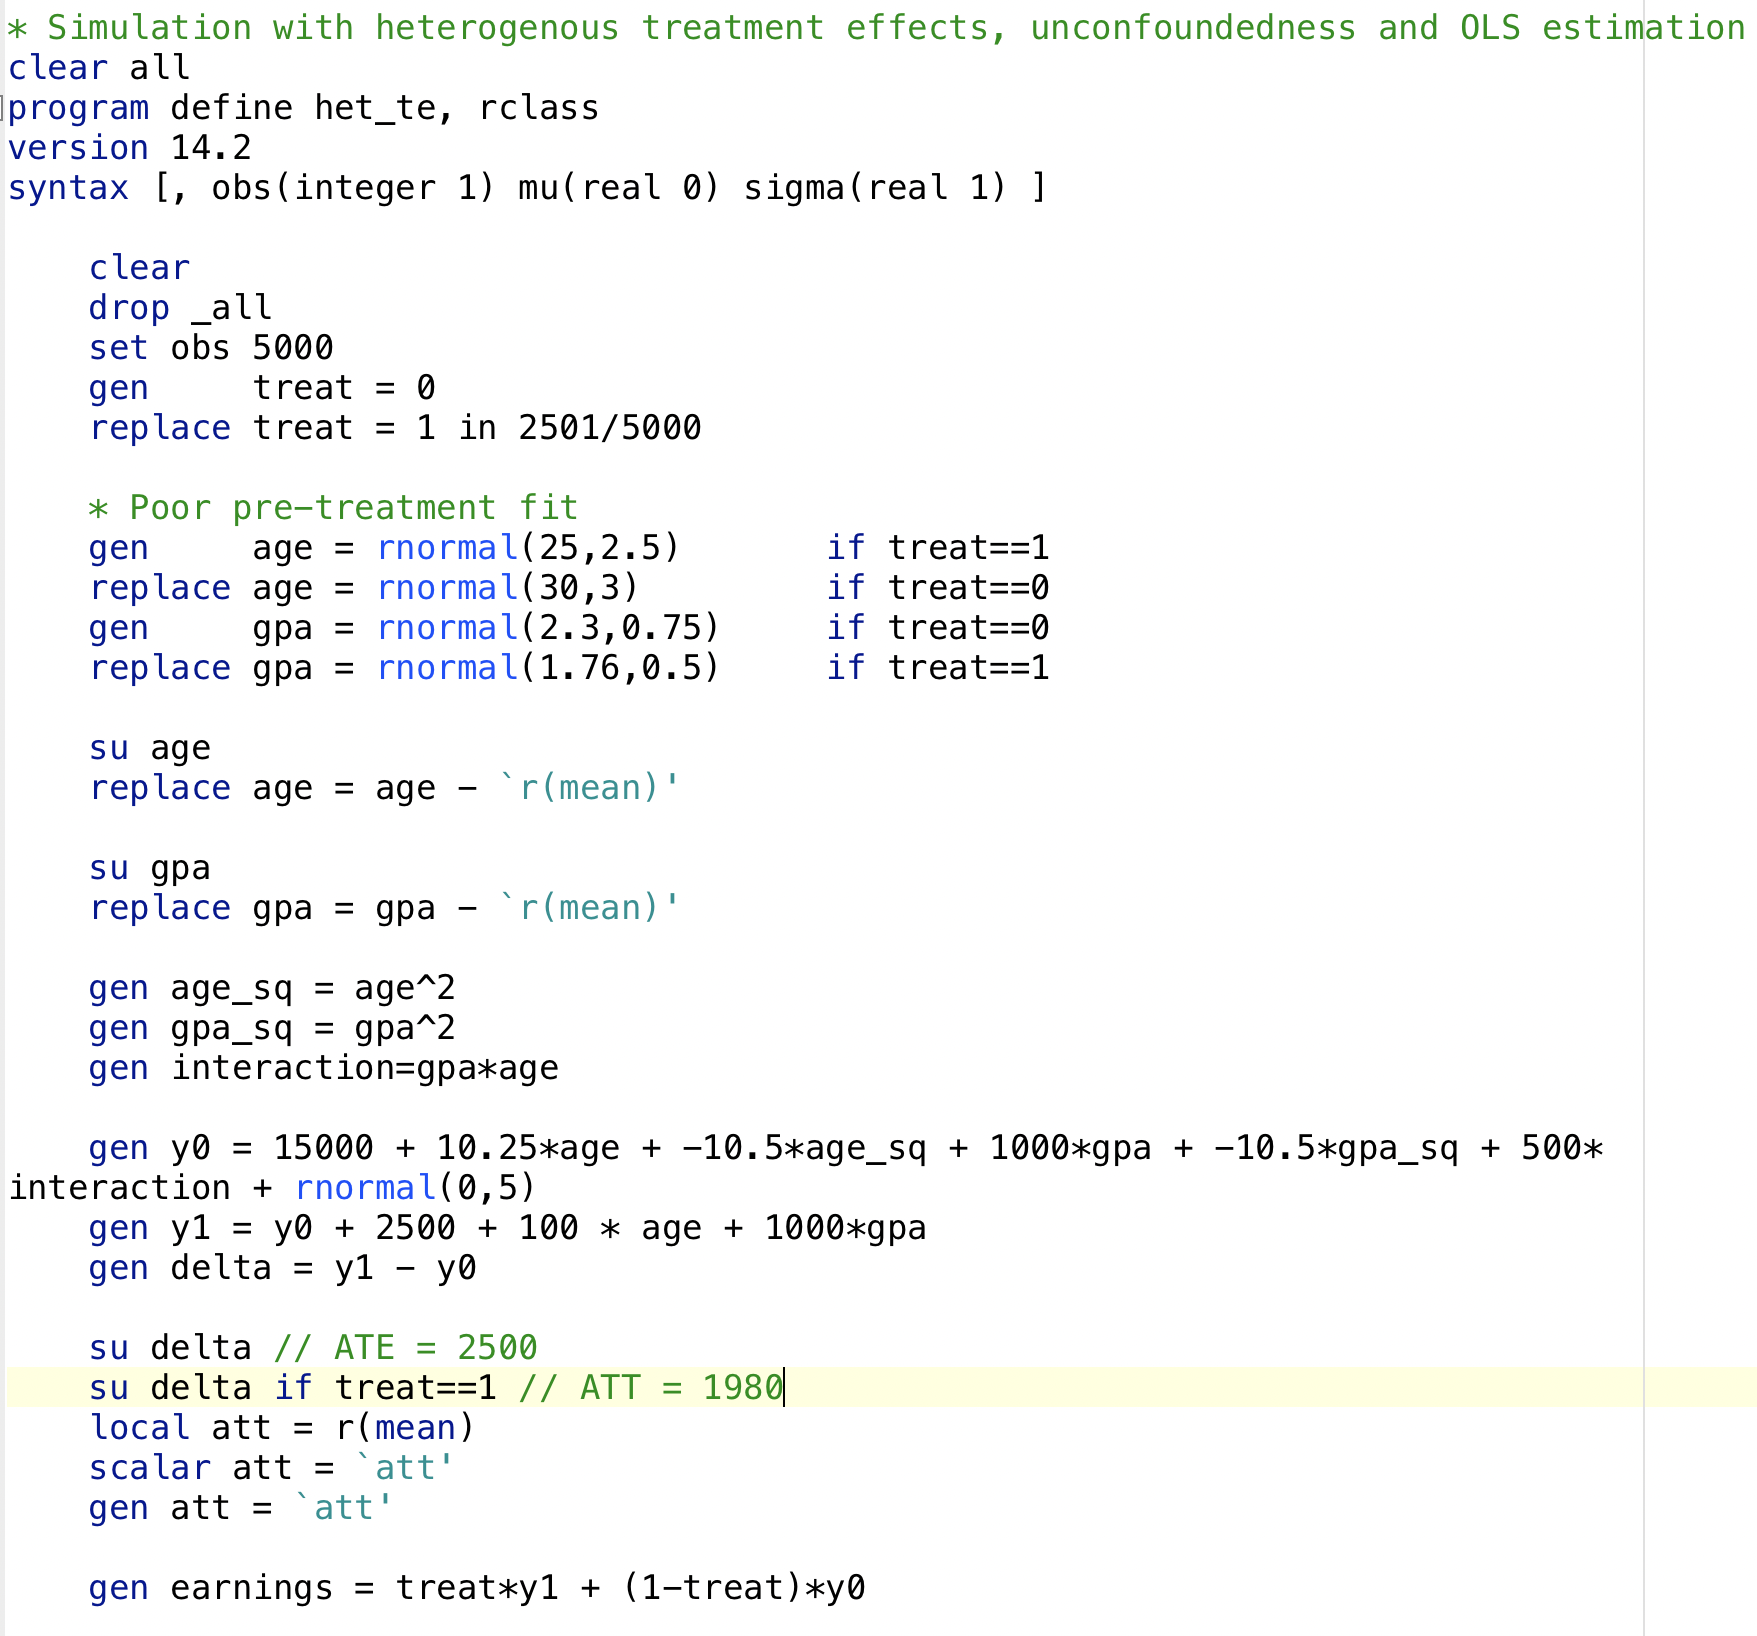
\includegraphics[scale=0.27]{./lecture_includes/stata_matching_code}
\end{figure}

\end{frame}

\begin{frame}{Parameters}

\begin{itemize}

\item We have two parameters: the ATE is \$2500 but the ATT is \$1980
\item What is the specification for each of them?
\item Let's look at what people usually do
\item 1,000 simulations of DGP with regression estimates plotting coefficient on treatment dummy: first with just age and GPA, second with the precise model used for $Y^0$ (but not $Y^1$)

\end{itemize}

\end{frame}


\begin{frame}{Constant Treatment Effects and Linearity}

\begin{figure}[!t]\centering
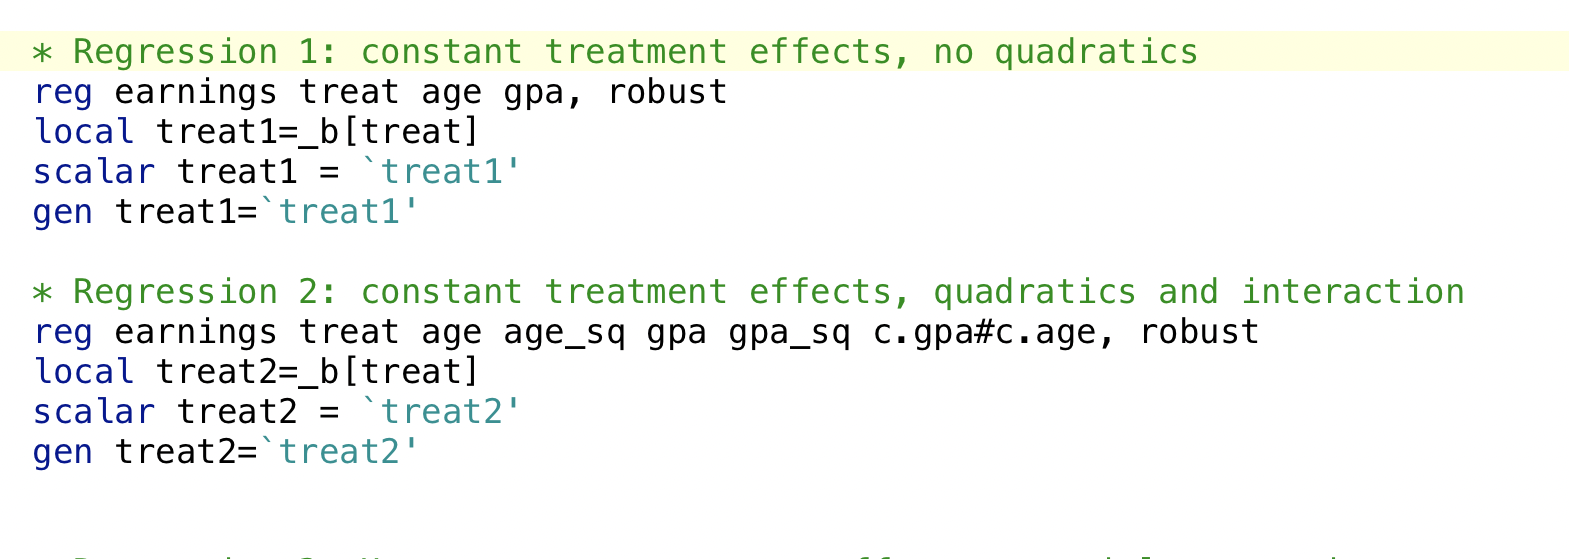
\includegraphics[scale=0.45]{./lecture_includes/stata_reg_constant}
\end{figure}

\end{frame}


\begin{frame}{Coefficient on Treatment Dummy is Wrong}

\begin{figure}[!t]\centering
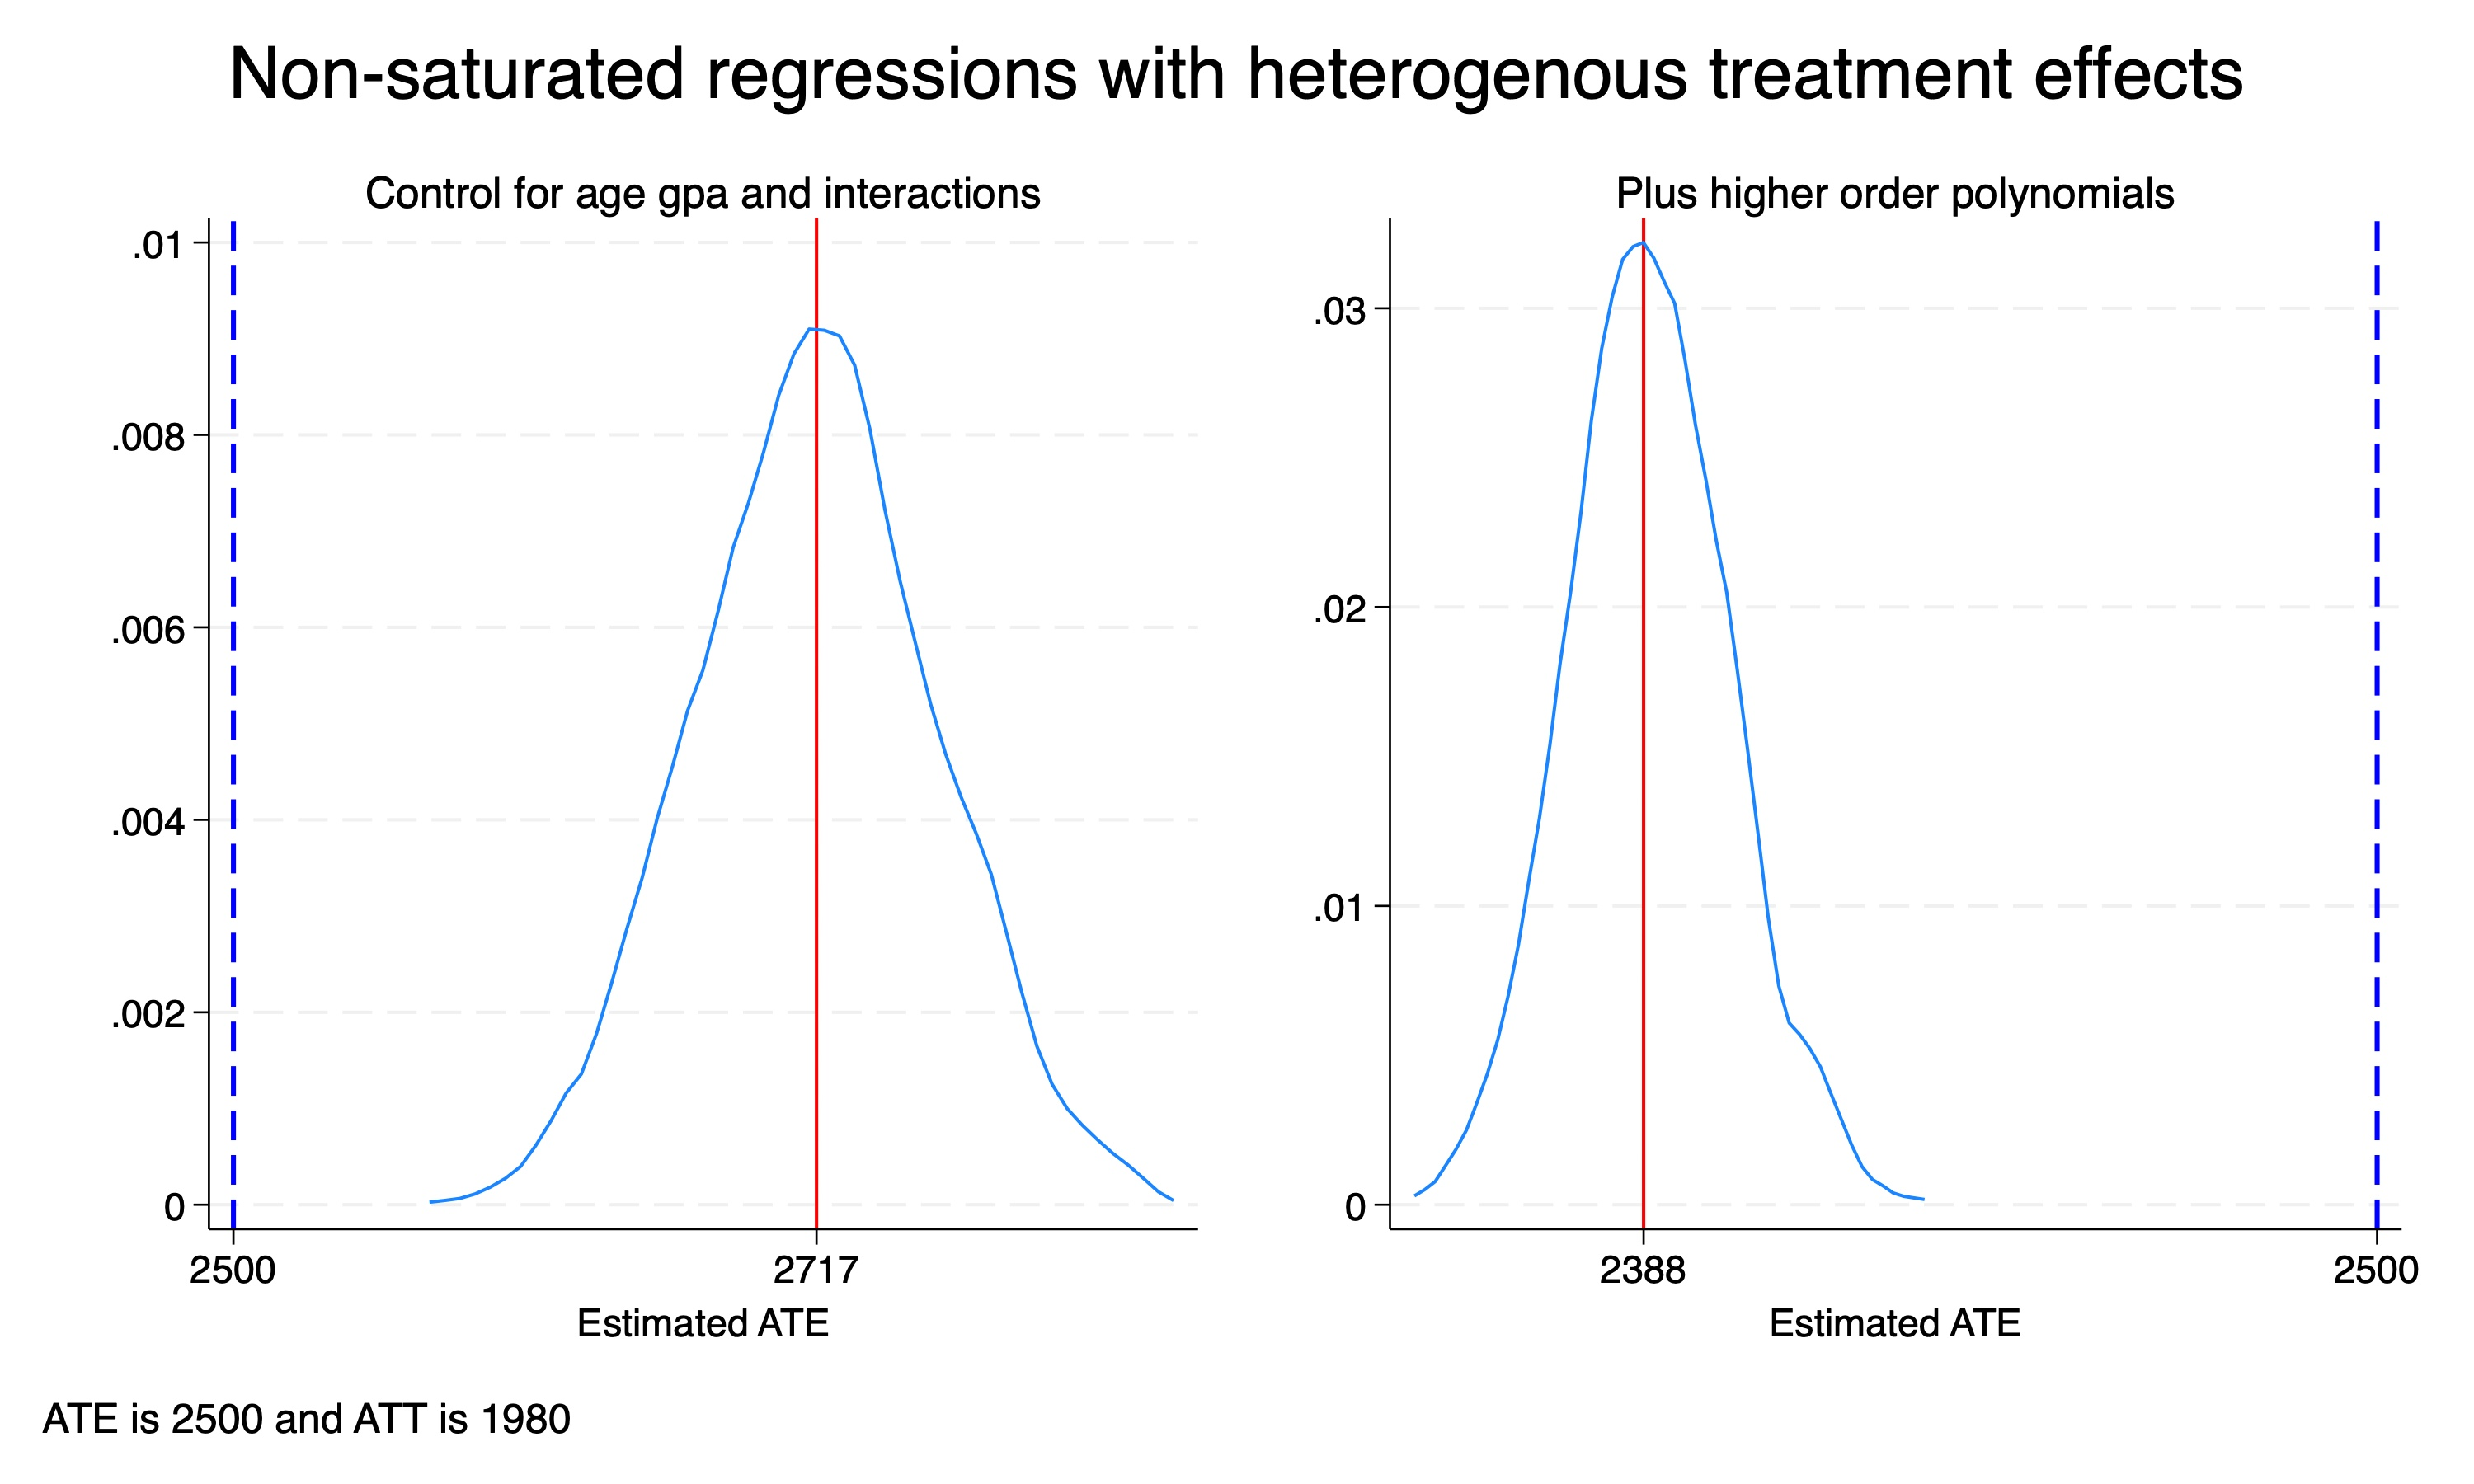
\includegraphics[scale=0.1]{./lecture_includes/combined_kernels.jpg}
\end{figure}

\end{frame}

\begin{frame}{Commentary}

\begin{itemize}

\item Three ifs and a then:

	\begin{itemize}
	\item \emph{If} unconfoundedness held, and 
	\item \emph{if} the potential outcome model was linear, and
	\item  \emph{if} the treatment effect had been homogenous with respect to age and GPA, 
	\item \emph{then} the coefficient on the treatment variable would have been the ATE 
	\end{itemize}
	
\item But it wasn't because homogeneity with respect to $X$ was not true (recall $Y(0)$ coefficients were not the same as $Y(1)$ coefficients)
\item Why were these models biased?  Didn't we have the correct specification in the second graph? 
\end{itemize}

\end{frame}

\begin{frame}{Heterogenous treatment effects}

Write down a simplified version of the DGP from the code:

\begin{eqnarray*}
Y^0_i &=& \alpha + \beta_{01} X_i + \varepsilon_i \\
Y^1_i &=& \alpha + \beta_{01} X_i + \delta D_i + \beta_{11} X_i \times D_i + \varepsilon_i
\end{eqnarray*}

\bigskip

Notice that the setup before, $X_i$ had a different effect on $Y^0$ than it did on $Y_i^1$ -- that's because of heterogenous treatment effects with respect to conditioning set. 

\end{frame}

\begin{frame}{Heterogenous treatment effects}

Take conditional expectations of the \emph{potential} outcomes:

\begin{eqnarray*}
E[Y^0_i | D_i=1, X_i] &=& \alpha + \beta_{01} E[X_i | D_i = 1, X_i] \\
E[Y^1_i | D_i=1, X_i] &=& \alpha + \beta_{01} E[X_i | D_i = 1, X_i]  \\
&& + \delta + \beta_{11} E[X_i | D_i=1,X_i]
\end{eqnarray*}

\bigskip

Average treatment effect is: 

\bigskip

\footnotesize

\begin{eqnarray*}
E[Y_i^1 | D_i, X^1_i] - E[Y^0_i | D_i, X_i] &=& \bigg (  \alpha + \beta_{01} E[X_i] + \delta + \beta_{11} E[X_i \times D_i | D_i=1,X_i] \bigg ) \\
&& -  \bigg (\alpha + \beta_{01} E[X_i] \bigg ) \\
&=& \delta + \beta_{11}  E[X_i \times D_i | D_i=1] 
\end{eqnarray*}OLS model accounting for heterogeneity must be ``fully saturated''.


\end{frame}




\begin{frame}{Regression adjustment}

This implies an interacted OLS model or what Wooldridge (2010) calls regression adjustment:

\bigskip

\begin{eqnarray*}
Y_i = \alpha + \delta D_i + \beta_{01} X_i + \beta_{11} D_i \times X_i + \varepsilon_i
\end{eqnarray*}

$\widehat{\delta}$ is the ATE but the ATT is equal to $\widehat{\delta} + \widehat{\beta_{11}} E[X_i | D_i = 1]$ where $E[X_i | D_i=1]$ is the sample average of $X_i$ for the treatment group

\bigskip

We will estimate two models: (1) once with simplified but incorrectly specified saturated and (2) another with the correctly specified saturated model -- warning, it's a huge pain and you can easily mess it up even with just a few variables

\end{frame}



\begin{frame}{Misspecified Saturated OLS Regression}

\begin{figure}[!t]\centering
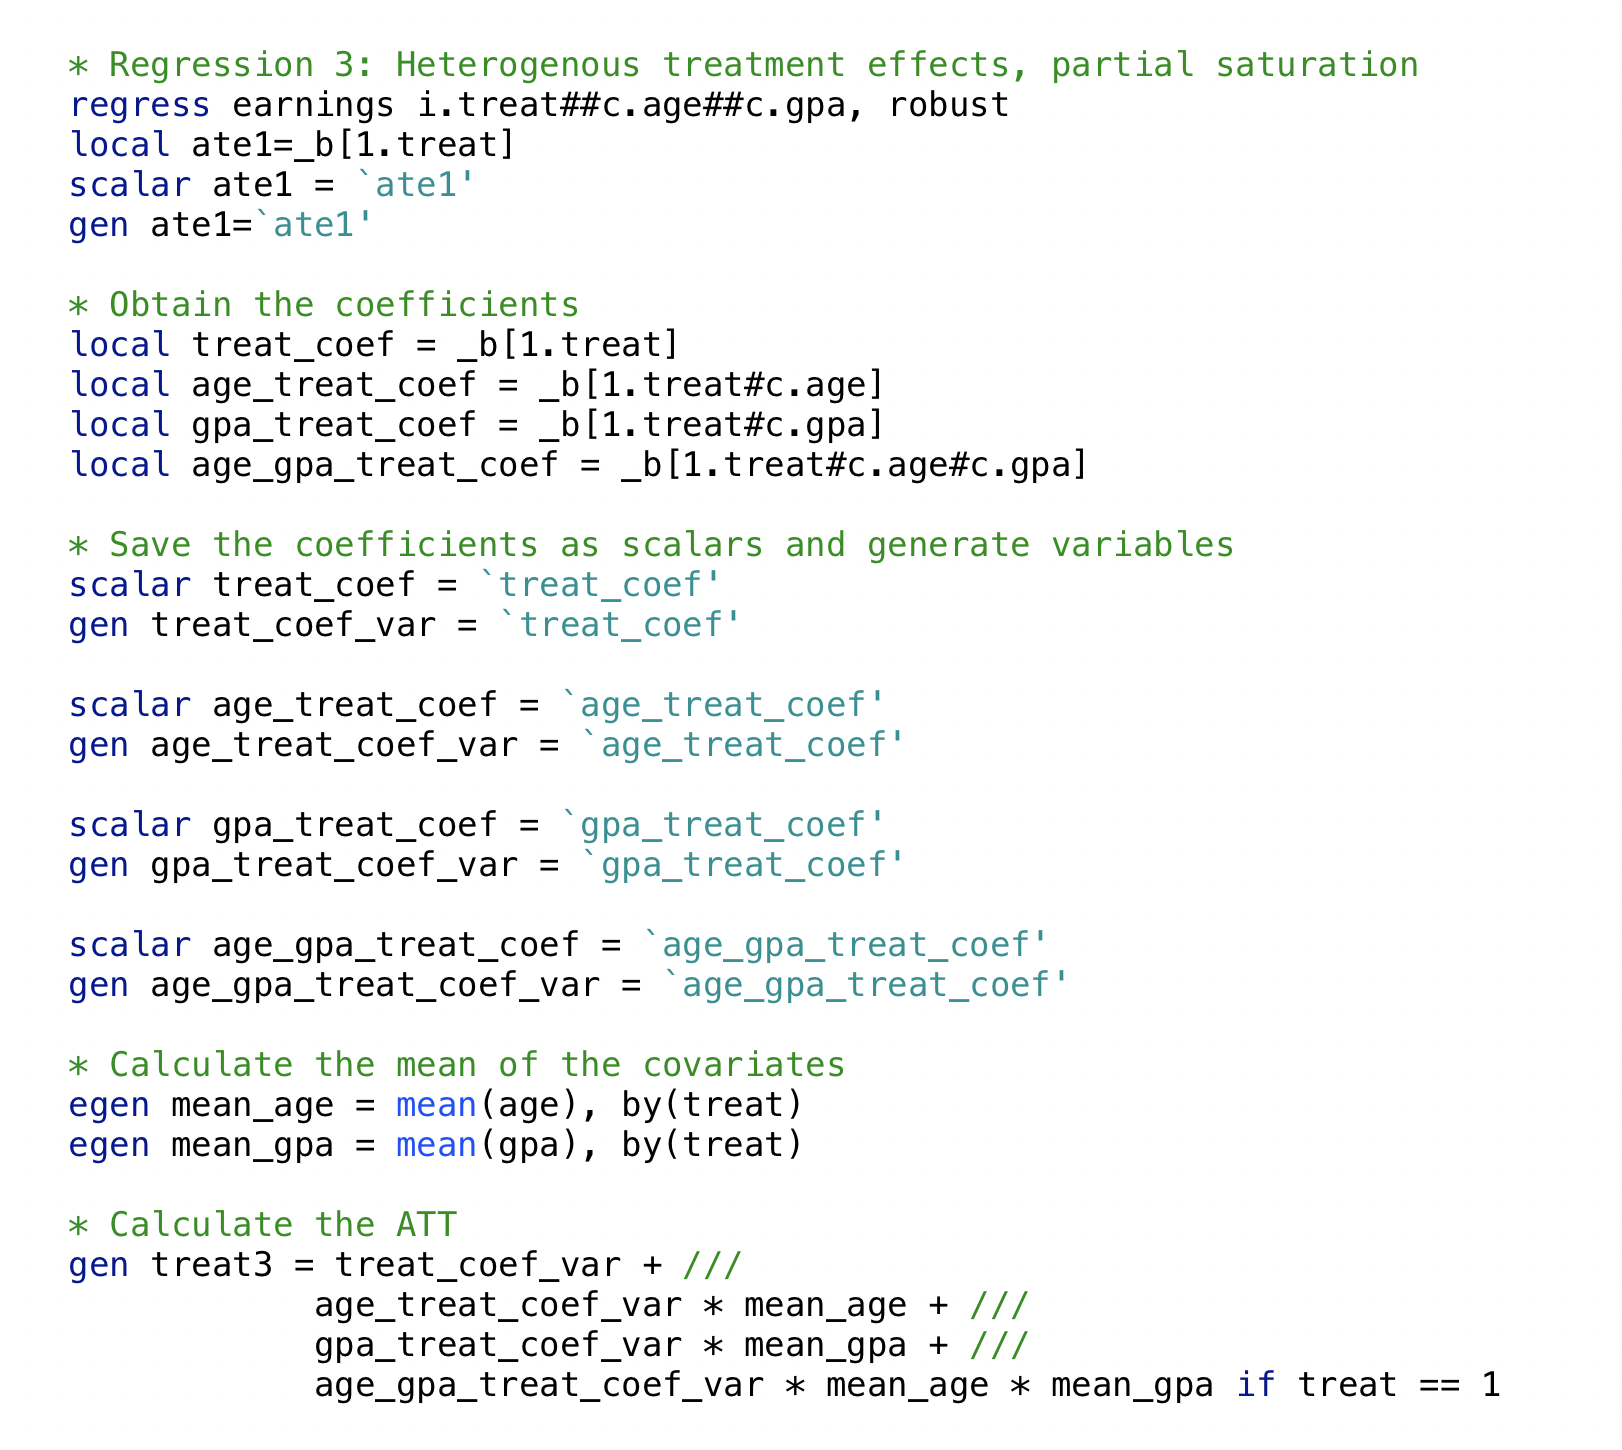
\includegraphics[scale=0.3]{./lecture_includes/saturated_reg3}
\end{figure}

\end{frame}


\begin{frame}{Misspecified Saturated OLS Regression}

\begin{figure}[!t]\centering
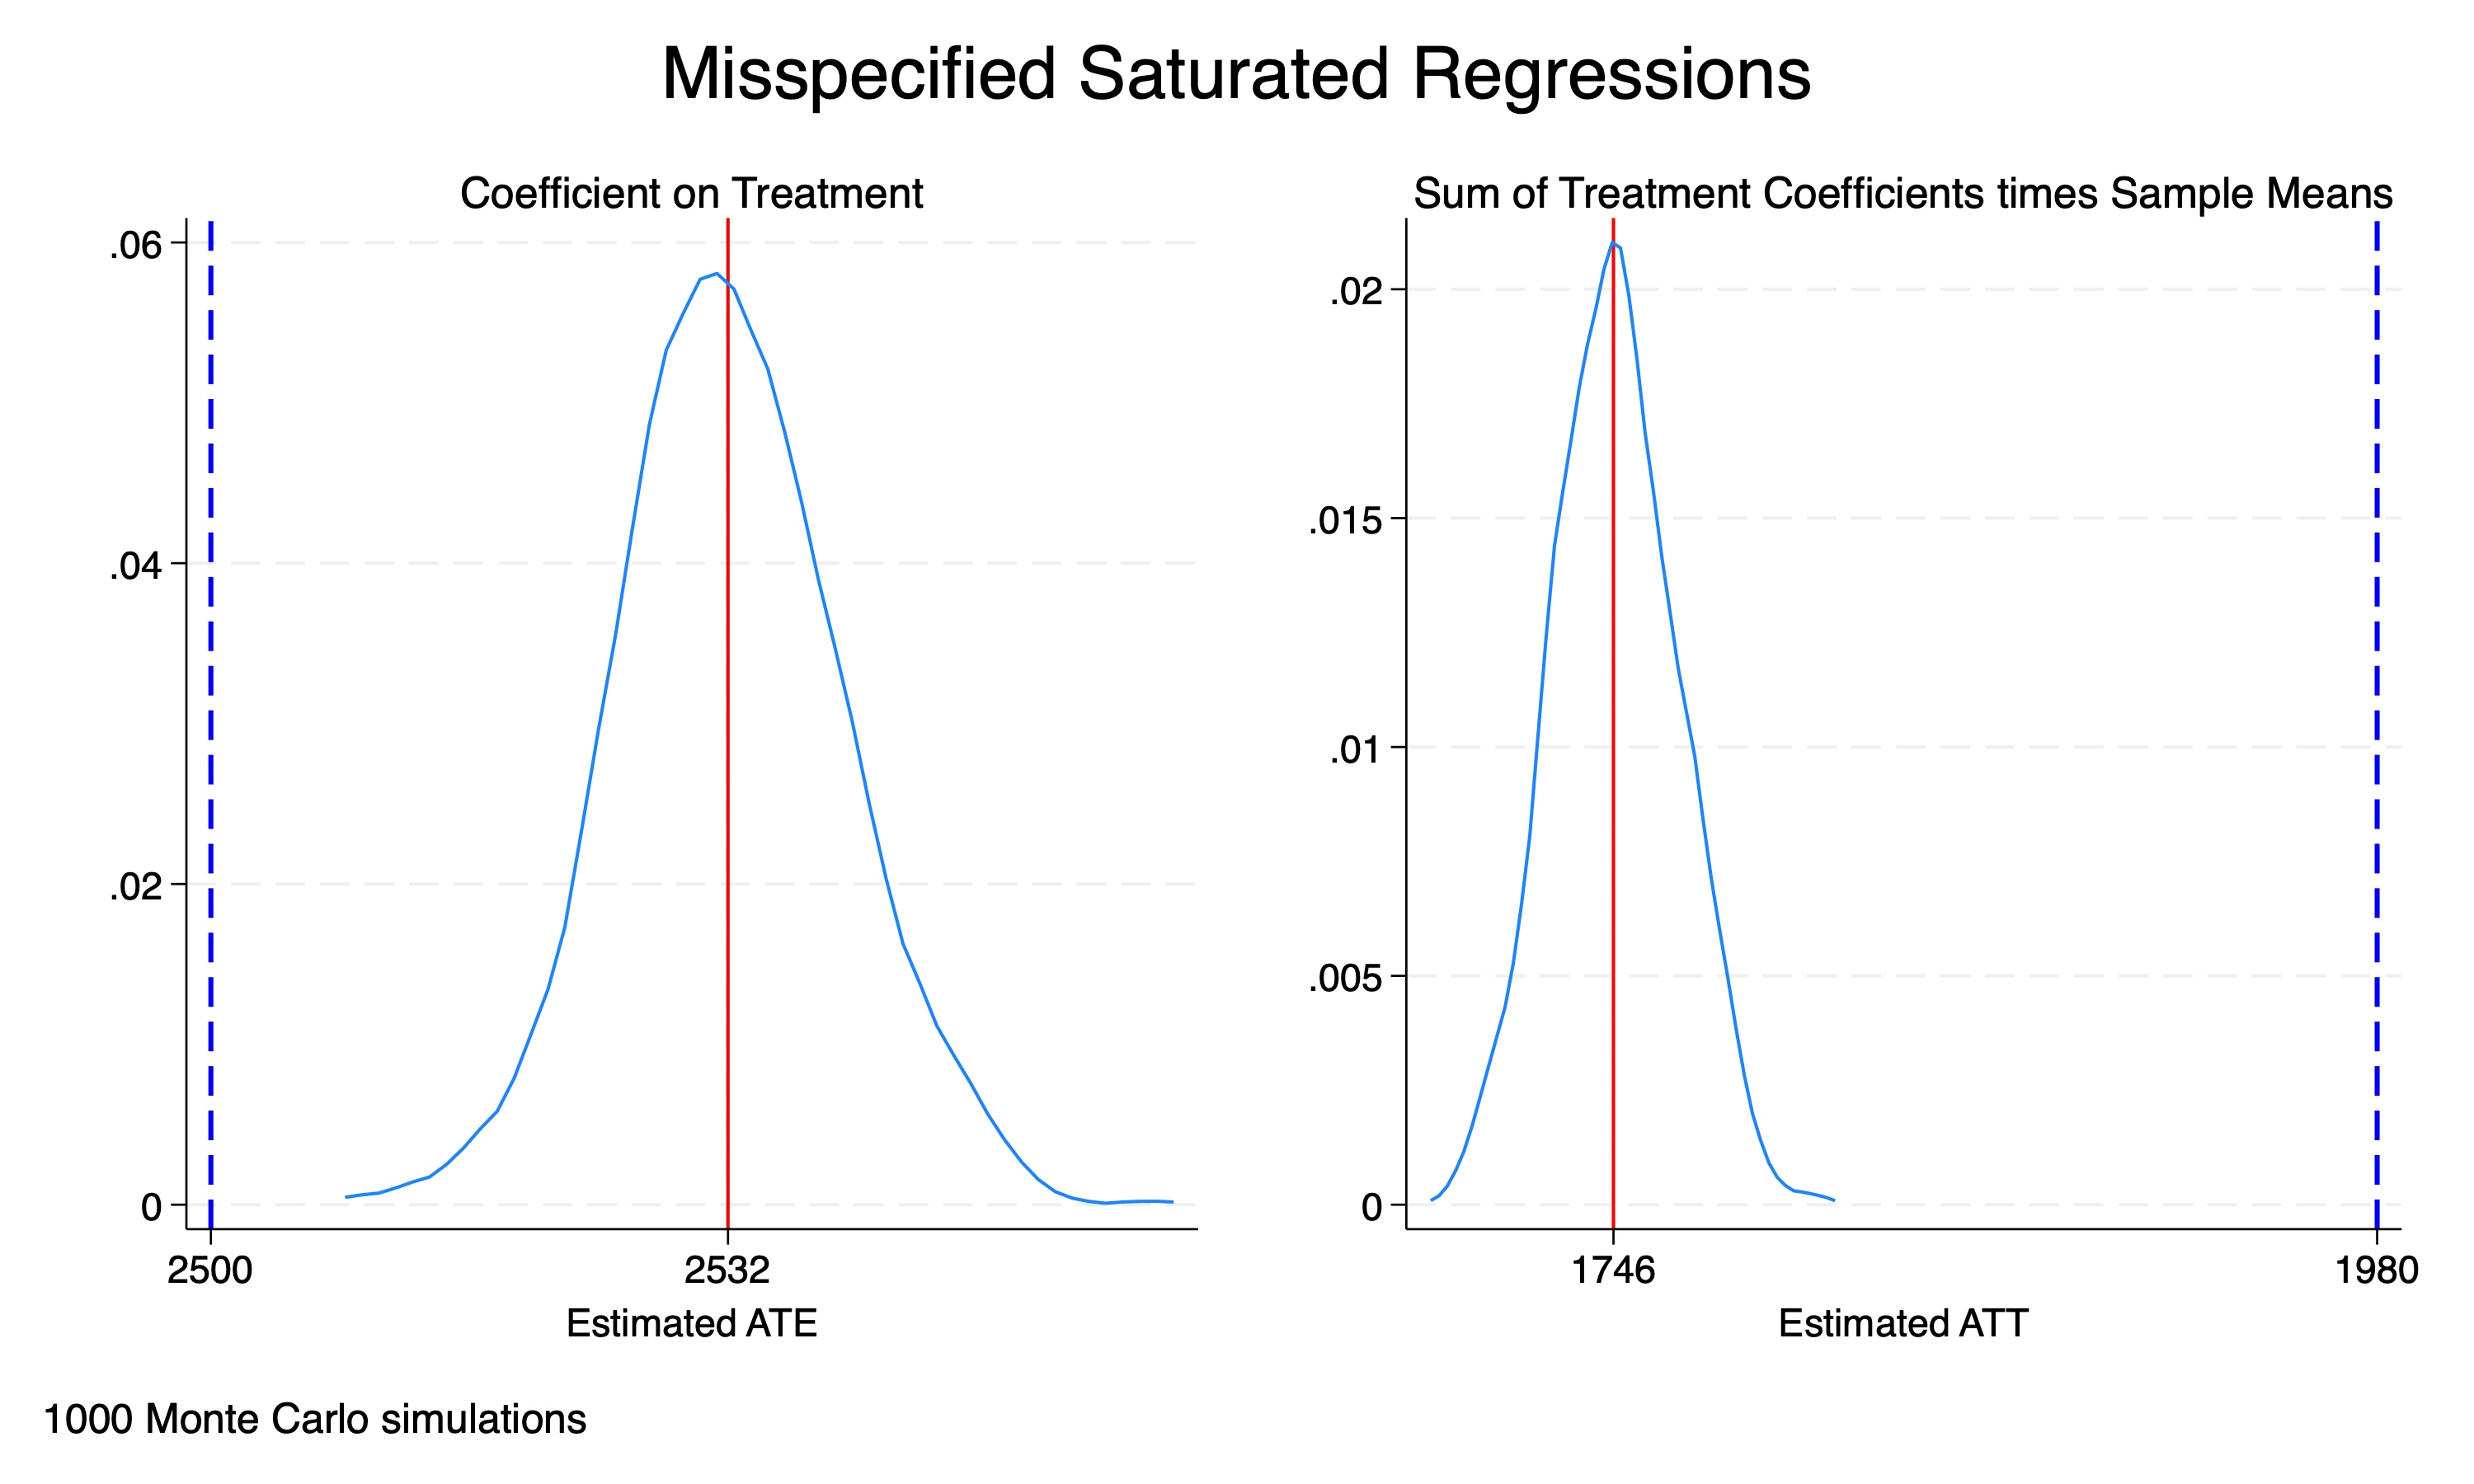
\includegraphics[scale=0.1]{./lecture_includes/combined_saturated1.jpg}
\end{figure}

\end{frame}

\begin{frame}{Comically Long Saturated OLS Regression}

\begin{figure}[!t]\centering
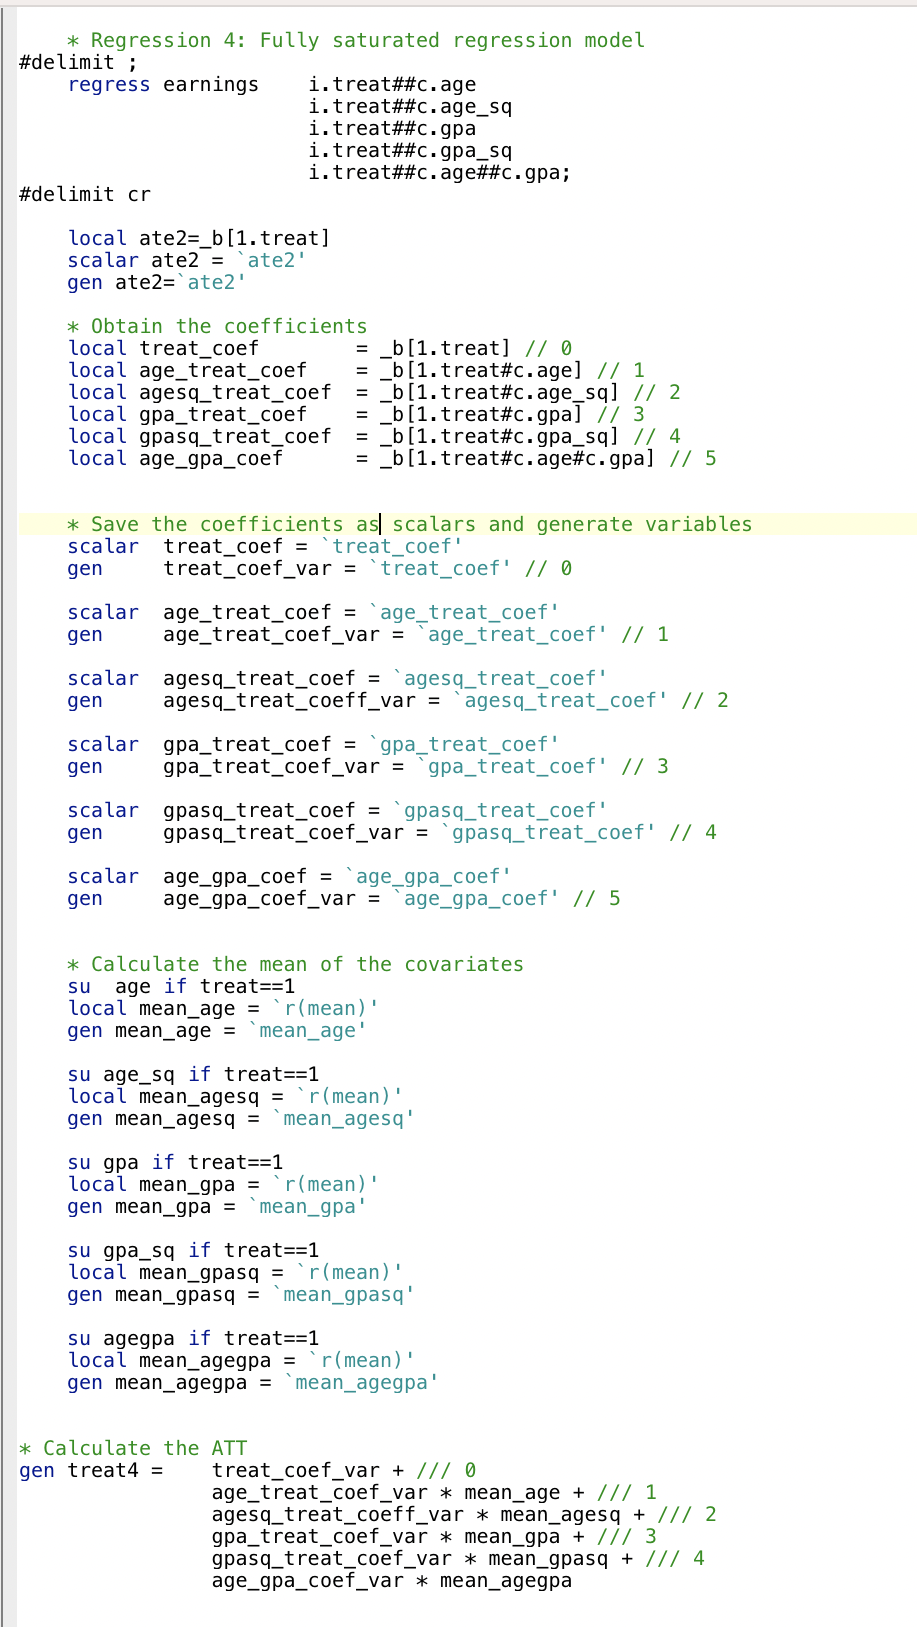
\includegraphics[scale=0.26]{./lecture_includes/stata_full_code}
\end{figure}

\end{frame}

\begin{frame}{Correctly Saturated OLS Regression}

\begin{figure}[!t]\centering
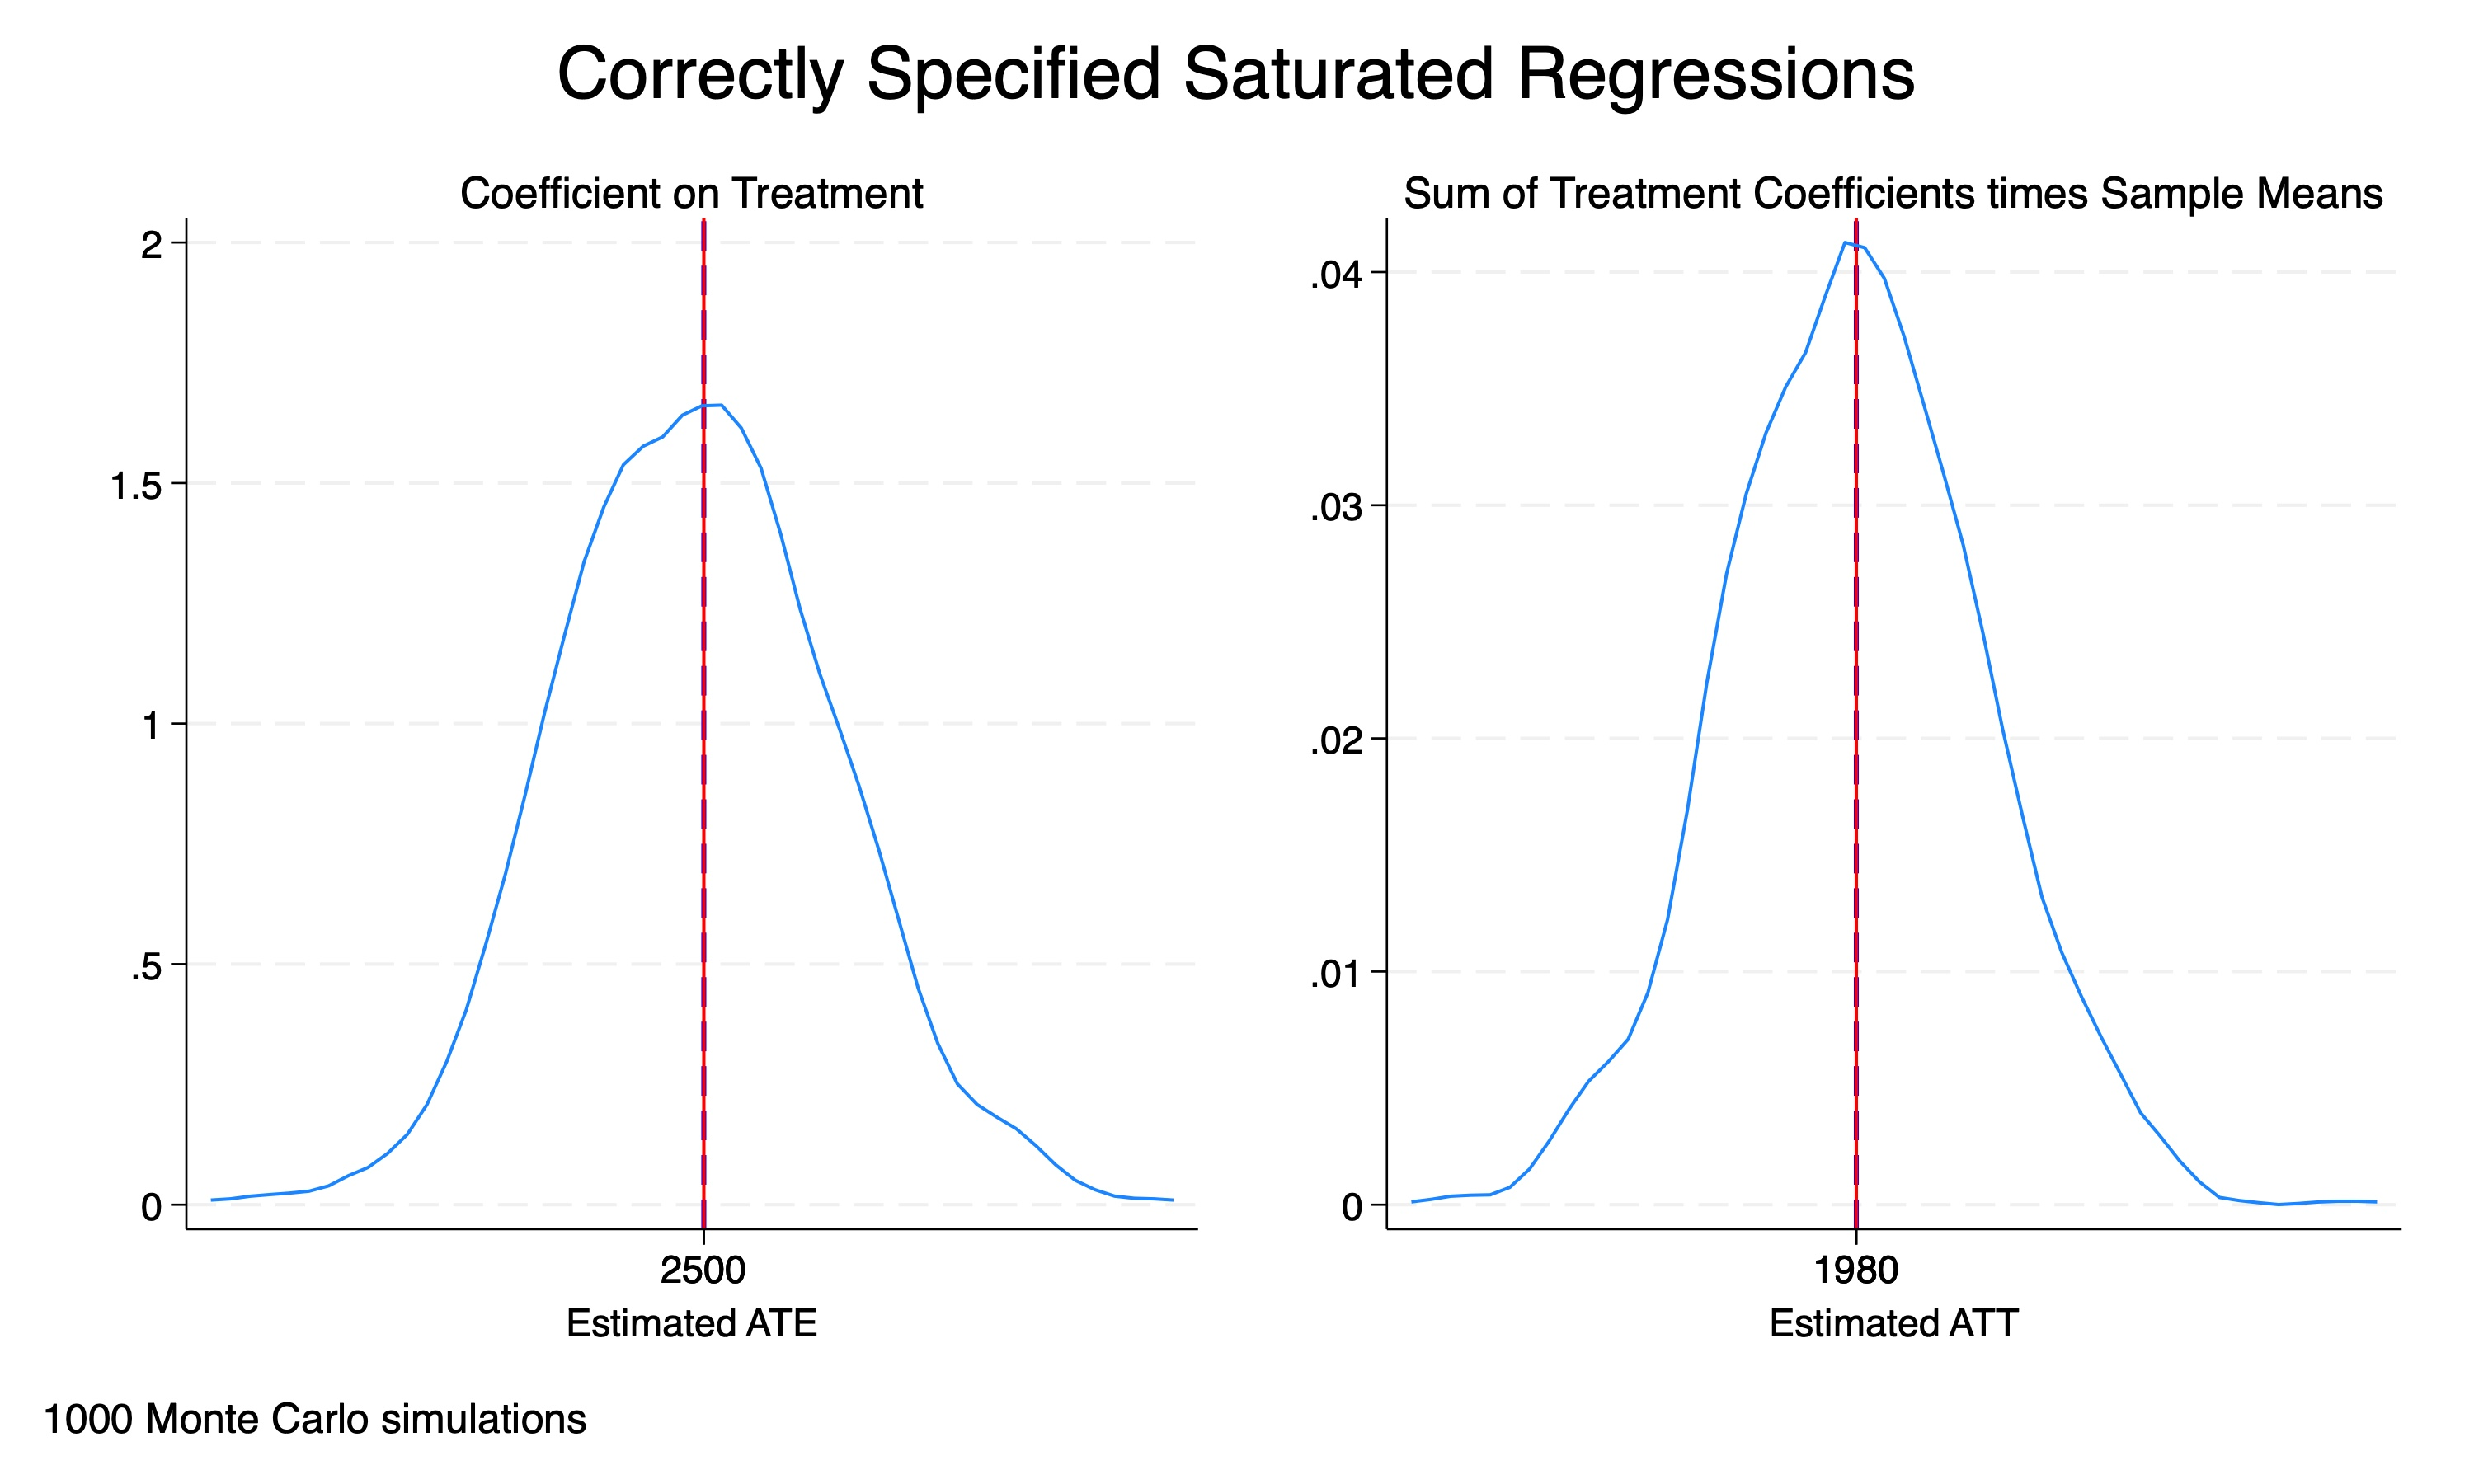
\includegraphics[scale=0.1]{./lecture_includes/combined_saturated2.jpg}
\end{figure}

\end{frame}

\begin{frame}{Regression adjustment}

\begin{itemize}

\item Notice how the same regression (fully interacted) led to \emph{both} the ATE and the ATT?
\item That means if you don't state ahead of time which parameter you want, how are you going to know how to set it up, and how will you know how to recover it?
\item Thankfully software exists that does this for you called ``regression adjustment'' by Wooldridge (2010) or Oaxaca-Blinder (Kline 2011; Graham and Pinto 2022) 
\item In Stata teffects, you can just the \texttt{ra} to get it -- see \texttt{comparison.do}

\end{itemize}

\end{frame}


\subsection{DML}


\begin{frame}{Curse of dimensionality and DML}

So recall our conversation then that we needed both unconfoundedness and common support, but you won't hear much about common support with DML because it extrapolates -- but there's some other reasons too

\begin{enumerate}
\item[1. ] Machine Learning Techniques: DML  incorporates machine learning methods that are robust to high-dimensional data. Methods like Lasso, Random Forests, or Gradient Boosting are designed to handle large numbers of features, potentially mitigating the curse of dimensionality to some extent.



\end{enumerate}

\end{frame}

\begin{frame}{Curse of dimensionality and DML}

\begin{enumerate}

\item[2. ] Double-Residualization: The double-residualization step in DML can help reduce dimensionality by focusing on the component of the outcome and treatment variable that cannot be explained by the high-dimensional controls (we'll see this in a second with the Frisch-Waugh-Lovell theorem)


\end{enumerate}

\end{frame}


\begin{frame}{Curse of dimensionality and DML}


\begin{enumerate}

\item[3. ] Sparsity: In many empirical applications, the true underlying model may be sparse, even if it's high-dimensional. Many machine learning techniques incorporated within DML are good at picking up this sparsity.  But what is sparsity in this context?

\end{enumerate}

\end{frame}

\begin{frame}{Sparsity in DML}

\begin{itemize}
\item \textbf{What is Sparsity?}: In high-dimensional models, sparsity refers to the property where only a small number of variables (features) have a significant impact on the outcome, even though there could be a large number of variables involved.

\end{itemize}

\end{frame}

\begin{frame}{Sparsity in DML}

\begin{itemize}

\item \textbf{Why is it Important?}
\begin{itemize}
\item \textit{Efficiency}: A sparse model reduces computational burden.
\item \textit{Interpretability}: Easier to focus on key variables, making the model more understandable.
\item \textit{Generalizability}: Sparse models are less likely to overfit, improving their performance on unseen data.
\end{itemize}

\end{itemize}

\end{frame}


\begin{frame}{Sparsity in DML}

\begin{itemize}

\item \textbf{DML and Sparsity}: Many machine learning techniques used within DML are adept at identifying these significant, non-zero parameters. Algorithms like LASSO, Random Forests, and certain neural networks can efficiently pick up this sparsity.
\end{itemize}

\end{frame}





\begin{frame}{Curse of dimensionality and DML}


\begin{enumerate}


\item[4. ] Regularization: Regularization methods used in machine learning can help to avoid overfitting, which is closely related to the curse of dimensionality. By penalizing the complexity of the model, regularization can help make the estimation problem more manageable, even in high dimensions.

\item[5. ]Cross-Fitting: This approach ensures that the model used to predict each observation is fitted on a separate sample, which can help to alleviate overfitting and, consequently, some issues related to high dimensionality.


\end{enumerate}

\end{frame}

\begin{frame}{Overfitting - The 'Overeager Student'}
\begin{itemize}
\item An overfit model performs exceedingly well on the data it's trained on, but poorly on new, unseen data.
\item Imagine a student who memorizes every question in the textbook but fails to understand the underlying concepts.
\item It’s like fitting a curve that passes through every data point, capturing noise as well as the trend.
\end{itemize}

\end{frame}


\begin{frame}
  \begin{figure}
    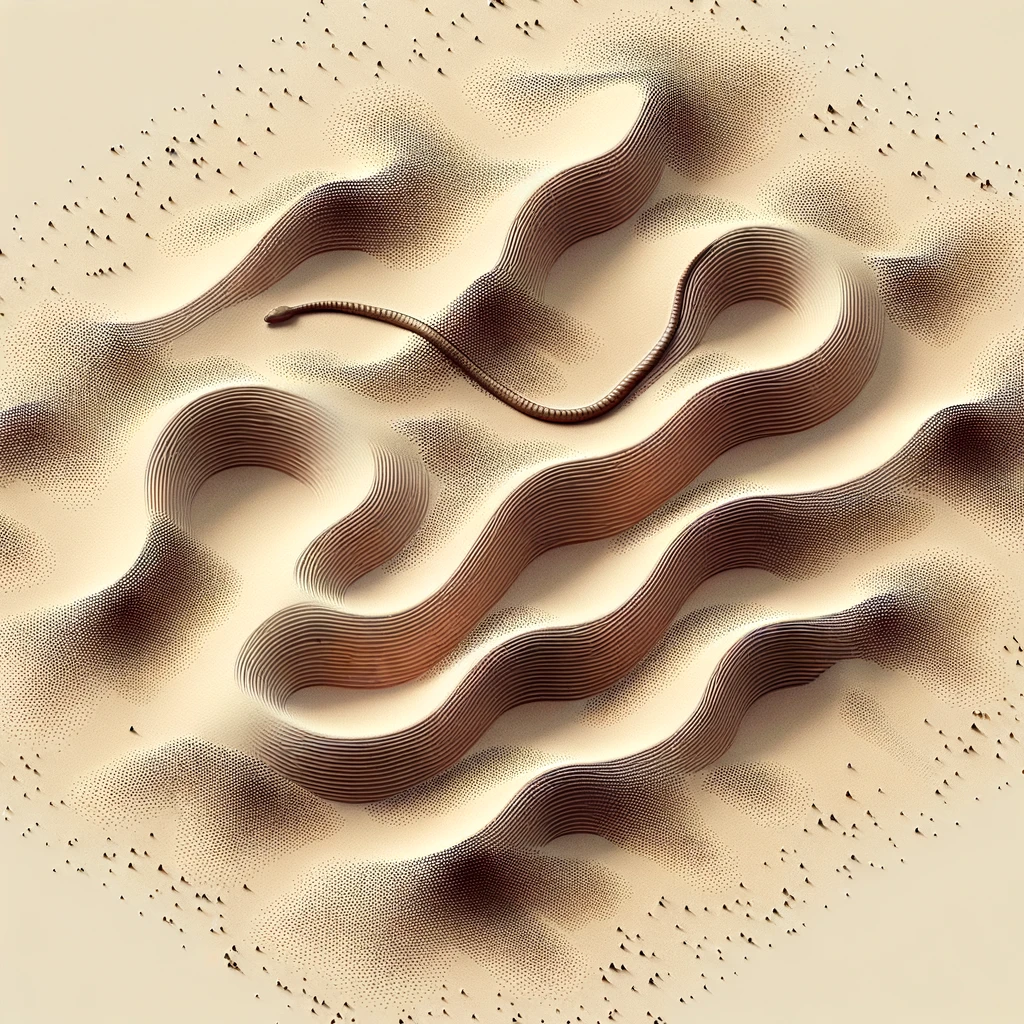
\includegraphics[scale=0.25]{./lecture_includes/overfit_snake.png}
  \end{figure}
\end{frame}


\begin{frame}{Underfitting - The 'Lazy Student'}
\begin{itemize}
\item Imagine a student who only studies the chapter titles, missing all the details.
\item An underfit model is too simple to capture the complexities in the data.
\item It performs poorly both on the data it was trained on and on new, unseen data.
\end{itemize}
\end{frame}


\begin{frame}
  \begin{figure}
    
\includegraphics[scale=0.25]{./lecture_includes/underfit_snake.png}
  \end{figure}
\end{frame}



\begin{frame}{The 'Goldilocks Zone' - Best Fitting}
\begin{itemize}
\item The ideal model is in the 'Goldilocks Zone': Not too simple, not too complex.
\item It performs well on both the training data and new, unseen data.
\item Balancing bias (systematic error) and variance (random error) is key to finding this sweet spot.
\end{itemize}
\end{frame}


\begin{frame}{Balancing Bias and Variance}
\begin{itemize}
\item \textbf{Bias}: Tendency of the model to consistently learn the wrong thing. High bias leads to underfitting.
\item \textbf{Variance}: Tendency of the model to be overly sensitive to fluctuations in the training data. High variance leads to overfitting.
\item The goal is to find a balance: Low bias and low variance, which equates to high accuracy on unseen data.
\end{itemize}
\end{frame}








\begin{frame}{Flexibility and Overfitting in ML}
  \textit{Credits: Facure's Online Book}
  \begin{itemize}
    \item The power you gain with ML is flexibility.
    \item ML can capture complicated functional forms in nuisance relationships.
    \item But this flexibility leads to the risk of overfitting.
  \end{itemize}
\end{frame}

\begin{frame}{Consequences of Overfitting}
  \begin{itemize}
    \item Overfitting causes residuals to be smaller than they should be.
    \item Overfitting captures not only the relationship between \( Y \) and \( X \) but also \( D \) and \( Y \), biasing the residual regression.
  \end{itemize}
\end{frame}

\begin{frame}{Overfitting and Treatment Variance}
  \begin{itemize}
    \item Overfitting can also affect the treatment variable.
    \item Reduced variance in treatment leads to higher variance in the final estimator.
    \item Violation of positivity can also have similar effects.
  \end{itemize}
\end{frame}

\begin{frame}{Cross Prediction and Out-of-Fold Residuals}
  \begin{itemize}
    \item Solution: Use cross prediction and out-of-fold residuals.
    \item Data is divided into \( K \) parts.
    \item Each part is estimated using the remaining \( K-1 \) parts to avoid driving residuals to zero.
  \end{itemize}
\end{frame}

\begin{frame}{Curse of dimensionality and DML}


\begin{enumerate}



\item[6. ]Interpretable Parameters: DML is often used to estimate a low-dimensional target (the treatment effect) while controlling for high-dimensional covariates. The curse of dimensionality is less of an issue when the parameter of interest is low-dimensional.

\end{enumerate}

\end{frame}


\begin{frame}{Summary and Next Steps}
  \begin{itemize}
    \item We've covered the challenges and solutions in using ML for DML.
    \item Next, let's dive into a step-by-step example with more technical discussion
  \end{itemize}
\end{frame}

\begin{frame}{Frisch-Waugh-Lovell}

\begin{itemize}
\item Old theorem showing that you can decompose a multivariate regression into a set of steps and get numerically the same number
\item Used by DML so we should review it, though it is more often called ``orthogonalized''
\end{itemize}

\end{frame}


\begin{frame}{OLS Simulated Code}

\begin{figure}[!t]\centering
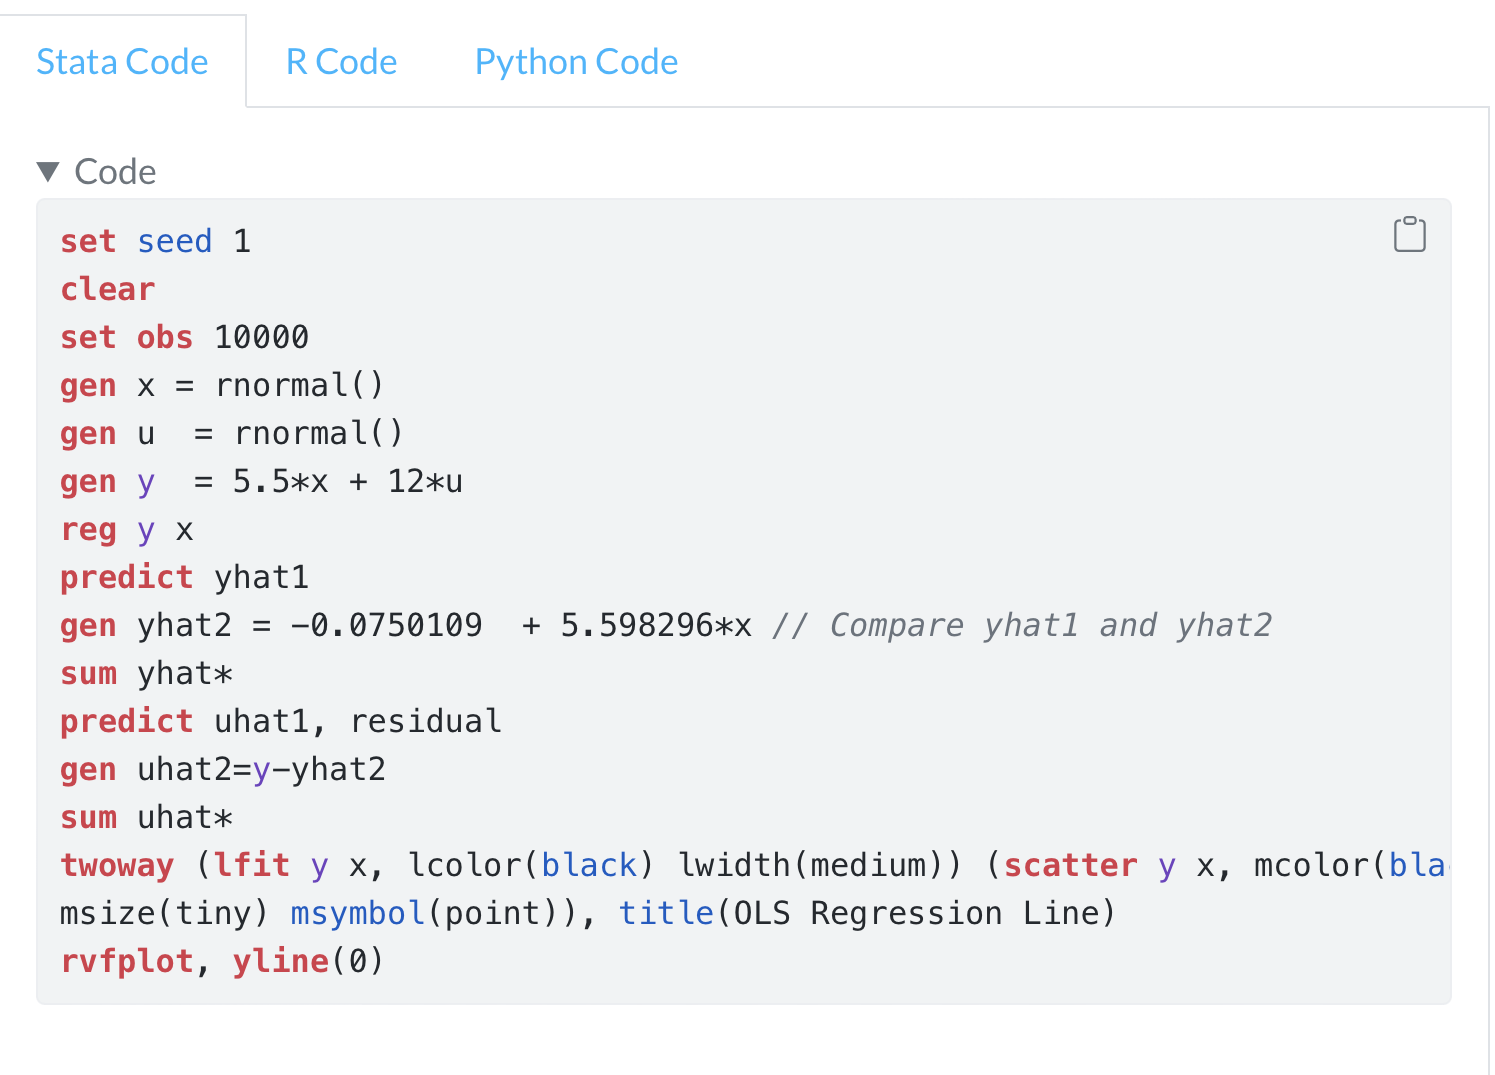
\includegraphics[scale=0.40]{./lecture_includes/ols_code}
\end{figure}

\end{frame}

\begin{frame}{OLS Plot and Line}

\begin{figure}[!t]\centering
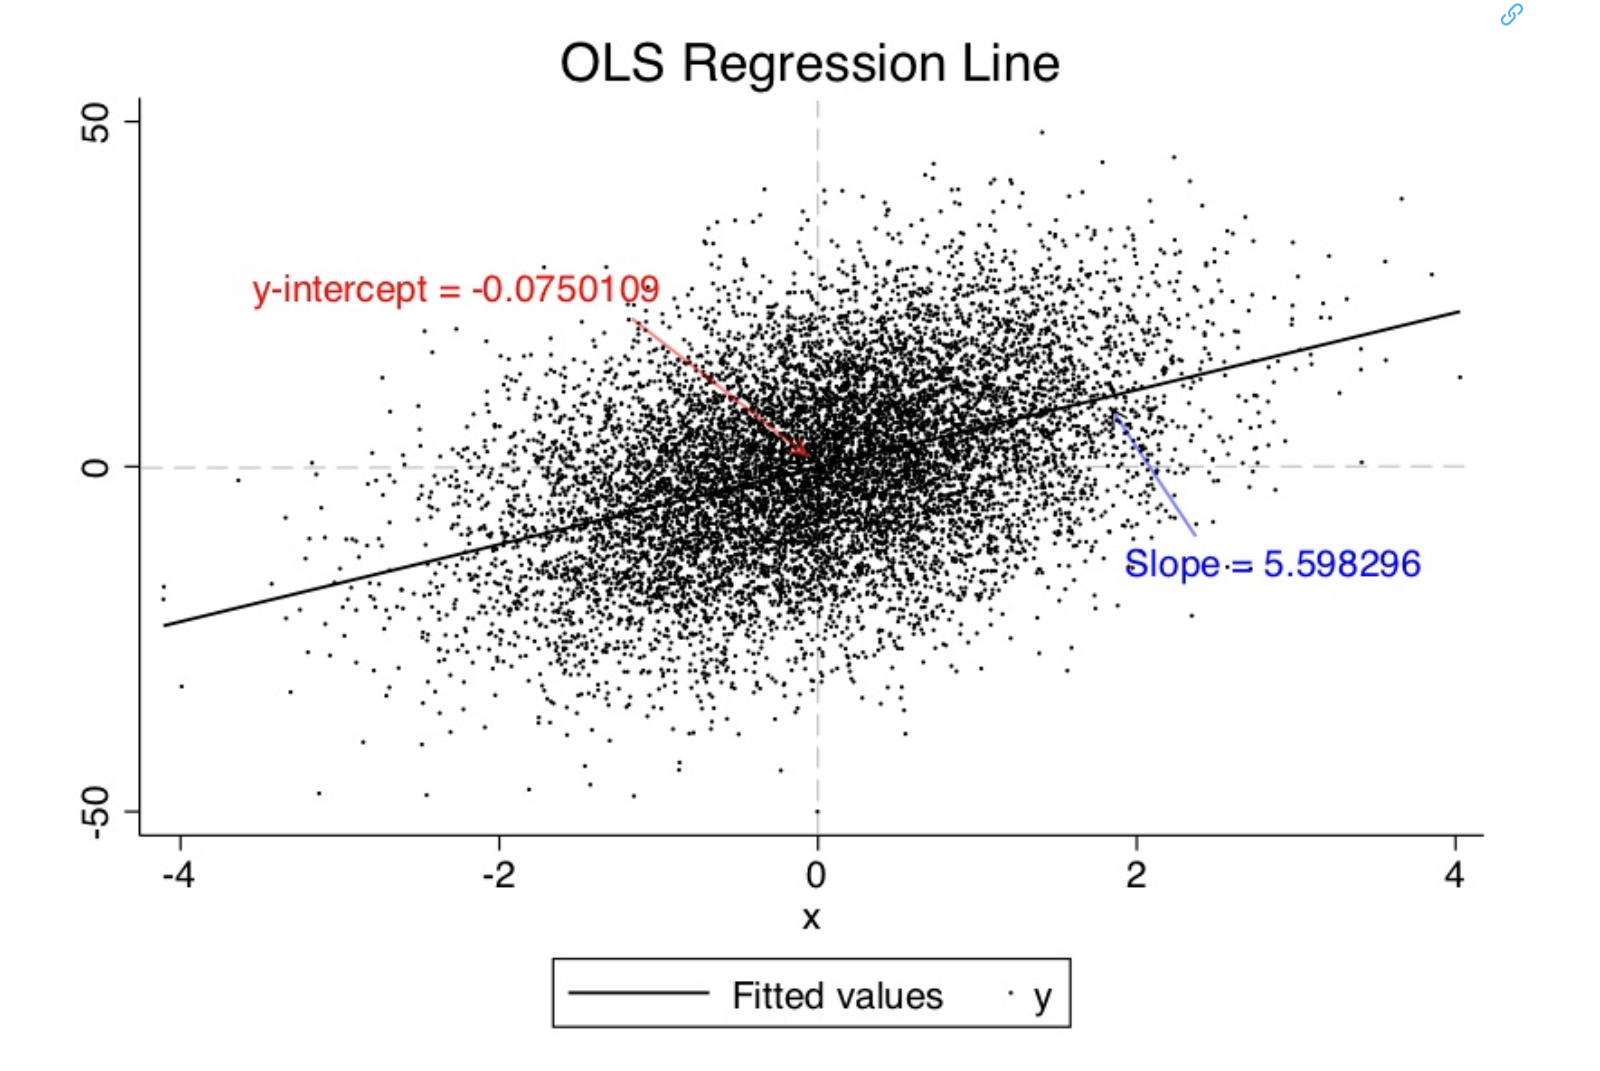
\includegraphics[scale=0.4]{./lecture_includes/ols_line}
\end{figure}

\end{frame}

\begin{frame}{Bivariate vs multivariate regressions}

\begin{itemize}

\item Interpreting the OLS coefficient in bivariate regression is written out as a scaled covariance:

 $$\widehat{\beta_1}=\frac{Cov(Y_i,X_i)}{Var(X_i)}$$
 
 \item But when we are looking at a multivariate regression, what is it?
 
 \end{itemize}
 
 \end{frame}
 
 \begin{frame}{Applying FWL theorem}

\begin{itemize}
\item Frisch-Waugh-Lovell also helps us interpret $\widehat{\beta}_1$ when there are covariates
 \item Use the FWL theorem to turn the multivariate regression coefficient into the simple bivariate one
\item Angrist and Pischke (2009) call FWL the ``regression anatomy theorem''
\item Filoso (2013) has an excellent proof
\end{itemize}

\end{frame}



\begin{frame}{Applying FWL theorem}

	\begin{itemize}
	\item Can we estimate the causal effect of family size on labor supply by regressing labor supply (\texttt{Y}) on family size (\texttt{X})?
		\begin{eqnarray*}
		Y_i = \beta_0 + \beta_1 X_i + u_i&\\
		\end{eqnarray*}
	\item If family size is random, then we can interpret $\widehat{\beta_1}$ as the ATE
	\item But how do we interpret $\widehat{\beta_1}$ if \texttt{family size} is only conditionally random?  
	\end{itemize}
\end{frame}


\begin{frame}{Applying FWL theorem}
	
	\begin{itemize}
	\item Assume the longer model is:
		\begin{eqnarray*}
Y_i &=& \beta_0 + \beta_1 X_i + \gamma_1 \texttt{White}_i + \gamma_2 \texttt{Married}_i \\
		& & + \gamma_3 \texttt{Age}_i + \gamma_4 \texttt{Employed}_i + u_i
		\end{eqnarray*}
	\item Assume unconfoundedness and constant treatment effects so that family size is independent conditional on all controls
	\item FWL shows that in a multivariate regression, any one coefficient fitted can be reconceived as a simple scaled covariance of the outcome and residualized treatment variable
	\end{itemize}
	
\end{frame}




		

\begin{frame}{FWL Theorem}

	\begin{block}{FWL Theorem }
	Assume your main multiple regression model of interest:$$y_i=\beta_0 + \beta_1x_{1i} + \dots + \beta_kx_{ki} + \dots + \beta_Kx_{Ki} + e_i$$ and an auxiliary regression in which the variable $x_{1i}$ is regressed on all the remaining independent variables$$x_{1i} = \gamma_0 + \gamma_{k-1}x_{k-1 i}+\gamma_{k+1}x_{k+1 i} + \dots + \gamma_Kx_{Ki}+f_i$$and $\tilde{x}_{1i} = x_{1i} - \widehat{x}_{1i}$ being the residual from the auxiliary regression. The parameter $\beta_1$ can be rewritten as:$$\beta_1=\frac{Cov(y_i,\tilde{x}_{1i})}{Var(\tilde{x}_{1i})}$$

	\end{block}

\end{frame}


\begin{frame}[plain, shrink=20]

\bigskip

	\begin{block}{FWL Proof  (Proof by Filoso 2013)}
	To prove the theorem, note $E[\tilde{x}_{ki}]=E[x_{ki}]-E[\widehat{x}_{ki}]=E[f_i]$, and plug $y_i$ and residual $\tilde{x}_{ki}$ from $x_{ki}$ auxiliary regression into the covariance $cov(y_i, \tilde{x}_{ki})$
	\begin{eqnarray*}
	\beta_k &=& \frac{ cov(y_i, \tilde{x}_{ki})}{var(\tilde{x}_{ki})} \\
			 &=& \frac{ cov(\beta_0 + \beta_1x_{1i} + \dots + \beta_kx_{ki} + \dots + \beta_Kx_{Ki} + e_i, \tilde{x}_{ki})}{var(\tilde{x}_{ki})} \\
			&=& \frac{ cov(\beta_0 + \beta_1x_{1i} + \dots + \beta_kx_{ki} + \dots + \beta_Kx_{Ki} + e_i,f_i)}{var(f_i)}
	\end{eqnarray*}
	\begin{enumerate}
	\item Since by construction $E[f_i]=0$, it follows that the term $\beta_0E[f_i]=0$.
	\item Since $f_i$ is a linear combination of all the independent variables with the exception of $x_{ki}$, it must be that$$\beta_1E[f_ix_{1i}] = \dots = \beta_{k-1}E[f_ix_{k-1 i}] = \beta_{k+1}E[f_ix_{k+1 i}] = \dots = \beta_KE[f_ix_{KI}] = 0$$
	\end{enumerate}
	\end{block}
\end{frame}


\begin{frame}[plain, shrink=20]

	\begin{block}{FWL Proof  (Proof by Filoso 2013)}
		\begin{enumerate}\addtocounter{enumi}{2}
		\item Consider now the term $E[e_if_i]$.  This can be written as:
			\begin{eqnarray*}
			E[e_if_i] &=& E[e_if_i] \\
			&=& E[e_i\tilde{x}_{ki}] \\
			&=& E[e_i(x_{ki} - \widehat{x}_{ki})] \\
			&=& E[e_ix_{ki}] - E[e_i\tilde{x}_{ki}]
			\end{eqnarray*}Since $e_i$ is uncorrelated with any independent variable, it is also uncorrelated with $x_{ki}$: accordingly, we have $E[e_ix_{ki}]=0$. With regard to the second term of the subtraction, substituting the predicted value from the $x_{ki}$ auxiliary regression, we get$$E[e_i\tilde{x}_{ki}] = E[e_i(\widehat{\gamma_0} + \widehat{\gamma_1}x_{1i} + \dots + \widehat{\gamma}_{k-1}x_{k-1}i+\widehat{\gamma}_{k+1}x_{k+1 i} + \dots + \widehat{\gamma}_Kx_{Ki})]$$Once again, since $e_i$ is uncorrelated with any independent variable, the expected value of the terms is equal to zero.  Then, it follows $E[e_if_i]=0$.
		
		\end{enumerate}
	\end{block}

\end{frame}

\begin{frame}[plain, shrink=25]

	\begin{block}{FWL Proof  (Proof by Filoso 2013)}
		\begin{enumerate}\addtocounter{enumi}{3}
		\item The only remaining term is $E[\beta_kx_{ki}f_i]$ which equals $E[\beta_kx_{ki}\tilde{x}_{ki}]$ since $f_i=\tilde{x}_{ki}$. The term $x_{ki}$ can be substituted using a rewriting of the auxiliary regression model, $x_{ki}$, such that$$x_{ki} = E[x_{ki} | X_{-k}] + \tilde{x}_{ki}$$This gives
			\begin{eqnarray*}
			E[\beta_kx_{ki}\tilde{x}_{ki}] &=& E[\beta_kE[\tilde{x}_{ki}(E[x_{ki}|X_{-k}]+\tilde{x}_{ki})]] \\
			&=& \beta_kE[\tilde{x}_{ki}(E[x_{ki}|X_{-k}]+\tilde{x}_{ki})] \\
			&=&\beta_k\{E[\tilde{x}^2_{ki}] + E[(E[x_{ki}|X_{-k}]\tilde{x}_{ki})]\} \\
			&=& \beta_k var(\tilde{x}_{ki})
			\end{eqnarray*}which follows directly from the orthogonoality between $E[x_{ki} | X_{-k}]$ and $\tilde{x}_{ki}$. From previous derivations we finally get$$cov(y_i,\tilde{x}_{ki}) = \beta_kvar(\tilde{x}_{ki})$$which completes the proof. \qedhere
		\end{enumerate}
	\end{block}

\end{frame}

\begin{frame}{FWL}

\begin{itemize}
\item Let's review the FWL ``partialing out'' interpretation of OLS estimated $\widehat{\beta_1}$ in code
\item We will use the fwl.do at /Labs/Matching for this
\end{itemize}

\end{frame}





\begin{frame}{Flexible Regression Model}
  Consider the flexible regression model:
  \[
    Y_i = \tau D_i + g(X_i) + \epsilon_i
  \]
  Our goal is to estimate the treatment effect \( \tau \).
\end{frame}

\begin{frame}{DML Steps}
  \begin{enumerate}
    \item Predict \( Y_i \) using \( X_i \) with Machine Learning and compute the residuals: \( \tilde{Y} = Y - \hat{Y}_{\text{DML}} \)
    \item Predict \( D_i \) using \( X_i \) with Machine Learning and compute the residuals: \( \tilde{D} = D - \hat{D}_{\text{DML}} \)
    \item Regress \( \tilde{Y}_i \) on \( \tilde{D}_i \)
  \end{enumerate}
  Note: \( \hat{Y}_{\text{DML}} \) and \( \hat{D}_{\text{DML}} \) should be predictions generated by a machine learning model trained on a set of observations that does not include \( i \). We accomplish this via cross-fitting.
\end{frame}

\begin{frame}{DML and FWL}


\begin{itemize}
\item Frisch-Waugh-Lovell (FWL) theorem is often viewed as a precursor to the debiasing steps in DML. 
\item Essentially, FWL allows you to estimate partial effects by taking residuals. 
\item You first remove the effect of control variables, and then run a simple univariate regression on these "purified" residuals to get unbiased estimates. 
\item This is fundamentally what DML is doing but in a more flexible, nonparametric setting.
\end{itemize}

\end{frame}

\begin{frame}{Frisch-Waugh-Lovell (FWL) Theorem}
  Consider the multiple linear regression model:
  \[
    Y = X \beta + D \gamma + \epsilon
  \]
  Recall from earlier -- the FWL theorem tells us that we can obtain \( \gamma \) (effect of \( D \)) by:
  \begin{enumerate}
    \item Regressing \( D \) on \( X \) to get residuals \( \tilde{D} \)
    \item Regressing \( {Y} \) on \( \tilde{D} \) to get \( \gamma \)
  \end{enumerate}
\end{frame}

\begin{frame}{Connection to DML}
  Now consider the model
  \[
    Y_i = \tau D_i + g(X_i) + \epsilon_i
  \]
  The steps in DML closely resemble FWL but are designed for a flexible function \( g(x) \):
  \begin{enumerate}
    \item Regress \( Y_i \) on \( X_i \) using ML to get residuals \( \tilde{Y}_i \)
    \item Regress \( D_i \) on \( X_i \) using ML to get residuals \( \tilde{D}_i \)
    \item Regress \( \tilde{Y}_i \) on \( \tilde{D}_i \) to estimate \( \tau \)
  \end{enumerate}
  This extends FWL to a machine learning setting.
\end{frame}

\begin{frame}{Summary}
  \begin{itemize}
    \item Both FWL and DML focus on "purifying" the variables of interest by removing the influence of control variables.
    \item DML extends the logic of FWL to a flexible, nonparametric setting using machine learning methods.
    \item The core idea in both approaches is to focus on residuals, effectively controlling for confounders.
  \end{itemize}
\end{frame}




\begin{frame}{Cross-Fitting in DML}
  \begin{enumerate}
    \item Divide the sample into \( K \) folds.
    \item For \( k = 1, \ldots, K \)
    \begin{itemize}
      \item[a.] Train a model to predict \( Y \) given \( X \), leaving out observations \( i \) in fold \( k \): \( \hat{Y}_{-k}(x) \)
      \item[b.] Train a model to predict \( D \) given \( X \), leaving out observations \( i \) in fold \( k \): \( \hat{D}_{-k}(x) \)
      \item[c.] Form residuals \( \tilde{Y}_i = Y_i - \hat{Y}_{-k}(X_i) \) and \( \tilde{D}_i = D_i - \hat{D}_{-k}(X_i) \)
    \end{itemize}
    \item Regress \( \tilde{Y}_i \) on \( \tilde{D}_i \)
  \end{enumerate}
  \textbf{Caveats and considerations:}
  \begin{itemize}
    \item Use cross-validation to choose tuning parameters.
    \item For inference, use robust standard errors from the last step.
  \end{itemize}
\end{frame}

\begin{frame}{Role of Tuning Parameters in ML Models}
\begin{itemize}
\item Tuning parameters, also known as hyperparameters, control the complexity of the machine learning models used.
\item For example, in Lasso, the regularization term $\lambda$  is a tuning parameter.
\item These parameters are not learned from the data but must be set prior to the learning process.
\item Too high or too low values can lead to overfitting or underfitting.
\end{itemize}
\end{frame}

\begin{frame}{Cross-Validation for Tuning Parameter Selection}
\begin{itemize}
\item Cross-validation helps us to choose the optimal tuning parameters.
\item By splitting the data into training and validation sets multiple times, we can find the parameters that yield the best out-of-sample performance.
\item This makes the DML approach more robust.
\end{itemize}
\end{frame}

\begin{frame}{Why Out-of-Fold Prediction?}
\begin{itemize}
\item Using the same data for training and prediction can introduce bias.
\item Out-of-fold prediction ensures that each observation's residual is computed using a model that did not train on that observation.
\item This step is crucial for unbiased treatment effect estimation.
\end{itemize}
\end{frame}

\begin{frame}{Stability and Generalization in DML}
\begin{itemize}
\item Cross-validation ensures the model's findings are stable across different subsamples.
\item This adds an extra layer of validation and makes the findings more likely to generalize.
\end{itemize}
\end{frame}




\begin{frame}{What is K-Folding?}
  \begin{itemize}
    \item The dataset is randomly partitioned into \( K \) equally (or nearly equally) sized folds.
    \item One fold is used as the test set, and the remaining \( K-1 \) folds are used as the training set.
    \item This process is repeated \( K \) times, each time using a different fold as the test set.
  \end{itemize}
\end{frame}

\begin{frame}{Cross-Fitting in DML}
  \begin{itemize}
    \item In DML, cross-fitting helps to ensure that the model is not using the same observations for both training and testing.
    \item This is essential for unbiased estimation.
  \end{itemize}
\end{frame}

\begin{frame}{Cross-Fitting Illustrated}
  \begin{figure}
    \centering
    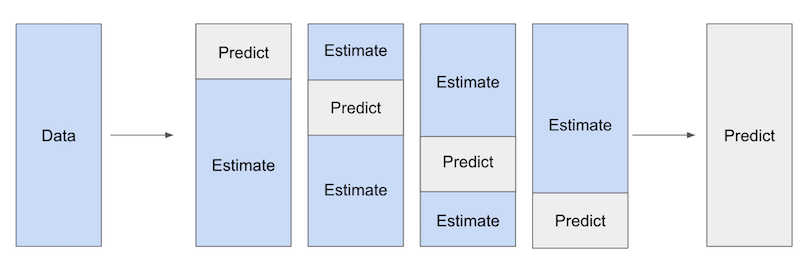
\includegraphics[width=0.8\textwidth]{./lecture_includes/facure-cross-prediction.png}
    \caption{An illustration of cross-fitting in DML}
  \end{figure}
\end{frame}



\begin{frame}{How Cross-Fitting Works in DML}
  \begin{enumerate}
    \item For each fold \( k \):
      \begin{itemize}
        \item Train the model on \( K-1 \) folds to predict \( Y \) and \( D \) based on \( X \).
        \item Use this trained model to predict the values in the left-out fold.
        \item Compute residuals \( \tilde{Y} \) and \( \tilde{D} \) for the left-out fold.
      \end{itemize}
    \item After looping through all \( K \) folds, you'll have residuals \( \tilde{Y} \) and \( \tilde{D} \) for all observations.
    \item Regress \( \tilde{Y} \) on \( \tilde{D} \) to obtain the treatment effect.
  \end{enumerate}
\end{frame}

\begin{frame}{Why Not Use All Observations?}
  \begin{itemize}
    \item Using the same data for both training and testing could lead to overfitting.
    \item Overfitting would bias our estimates and make them unreliable.
    \item Cross-fitting via k-folding helps to mitigate this by ensuring each observation is "out-of-sample" in one of the \( K \) iterations.
  \end{itemize}
\end{frame}

\begin{frame}{Role of Debiasing in DML}
  \textit{Credits: Facure's Online Book}
  \begin{itemize}
    \item Role of \( D \) model: Debiasing the treatment.
    \item Residuals \( \tilde{D} \) are treatment values where confounding bias has been removed.
    \item \( \tilde{D} \) is orthogonal to \( X \).
  \end{itemize}
\end{frame}

\begin{frame}{Example: Ice Cream and Temperature}
  \begin{itemize}
    \item In Facure's example with Ice Cream and Temperature:
    \item Residuals remove the influence of weekends on higher prices.
    \item This results in an unbiased representation of the treatment (price).
  \end{itemize}
\end{frame}

\begin{frame}{Role of Denoising in DML}
  \begin{itemize}
    \item Role of \( Y \) model: Denoising the outcome.
    \item It creates a version of the outcome where variance due to \( X \) has been explained.
    \item This makes causal estimation easier as the noise is reduced.
  \end{itemize}
\end{frame}

\begin{frame}{Summary}
  \begin{itemize}
    \item We've delved into the roles of debiasing and denoising in DML.
    \item These steps are crucial for unbiased and accurate causal estimation.
  \end{itemize}
\end{frame}


\begin{frame}{Conditional ATE in DML}
  \textit{Credits: Facure's Online Book}
  \begin{itemize}
    \item Double/Debiased ML is not limited to ATE.
    \item Can also be used to estimate Conditional Average Treatment Effect (CATE).
    \item Causal parameter changes based on unit's covariates.
  \end{itemize}
\end{frame}

\begin{frame}{Estimating CATE}
  \begin{itemize}
    \item Use the same residualized version of treatment and outcome.
    \item Interact these residuals with other covariates.
    \item Fit a linear CATE model.
  \end{itemize}
\end{frame}

\begin{frame}{Final Linear Model for CATE}
  \begin{itemize}
    \item Randomized test set used for CATE predictions.
    \item Final model is linear, enabling mechanical computation of CATE.
  \end{itemize}
\end{frame}

\begin{frame}{Generalization: R-Learner}
  \begin{itemize}
    \item This procedure is a general one.
    \item Known as R-Learner, inspired by the work of Robinson (1988).
    \item Emphasizes the role of residualization.
    \item New loss function defined, which can be minimized in various ways.
  \end{itemize}
\end{frame}

\begin{frame}{Summary}
  \begin{itemize}
    \item DML provides a flexible framework to estimate both ATE and CATE.
    \item CATE allows for nuanced treatment effect estimates based on covariates.
  \end{itemize}
\end{frame}


\section{Concluding remarks}

\begin{frame}{Buyer beware}
\begin{itemize}

\item Difficult paper to read; encourage you to read online material
\item Also remember the core assumptions remain: unconfoundedness
\item That means avoiding colliders and having all known and quantified confounders
\item Machine learning, including DML, can be ``naive'' too if the large dimension of features includes unknowingly colliders

\end{itemize}

\end{frame}

\begin{frame}{}

  \begin{figure}
    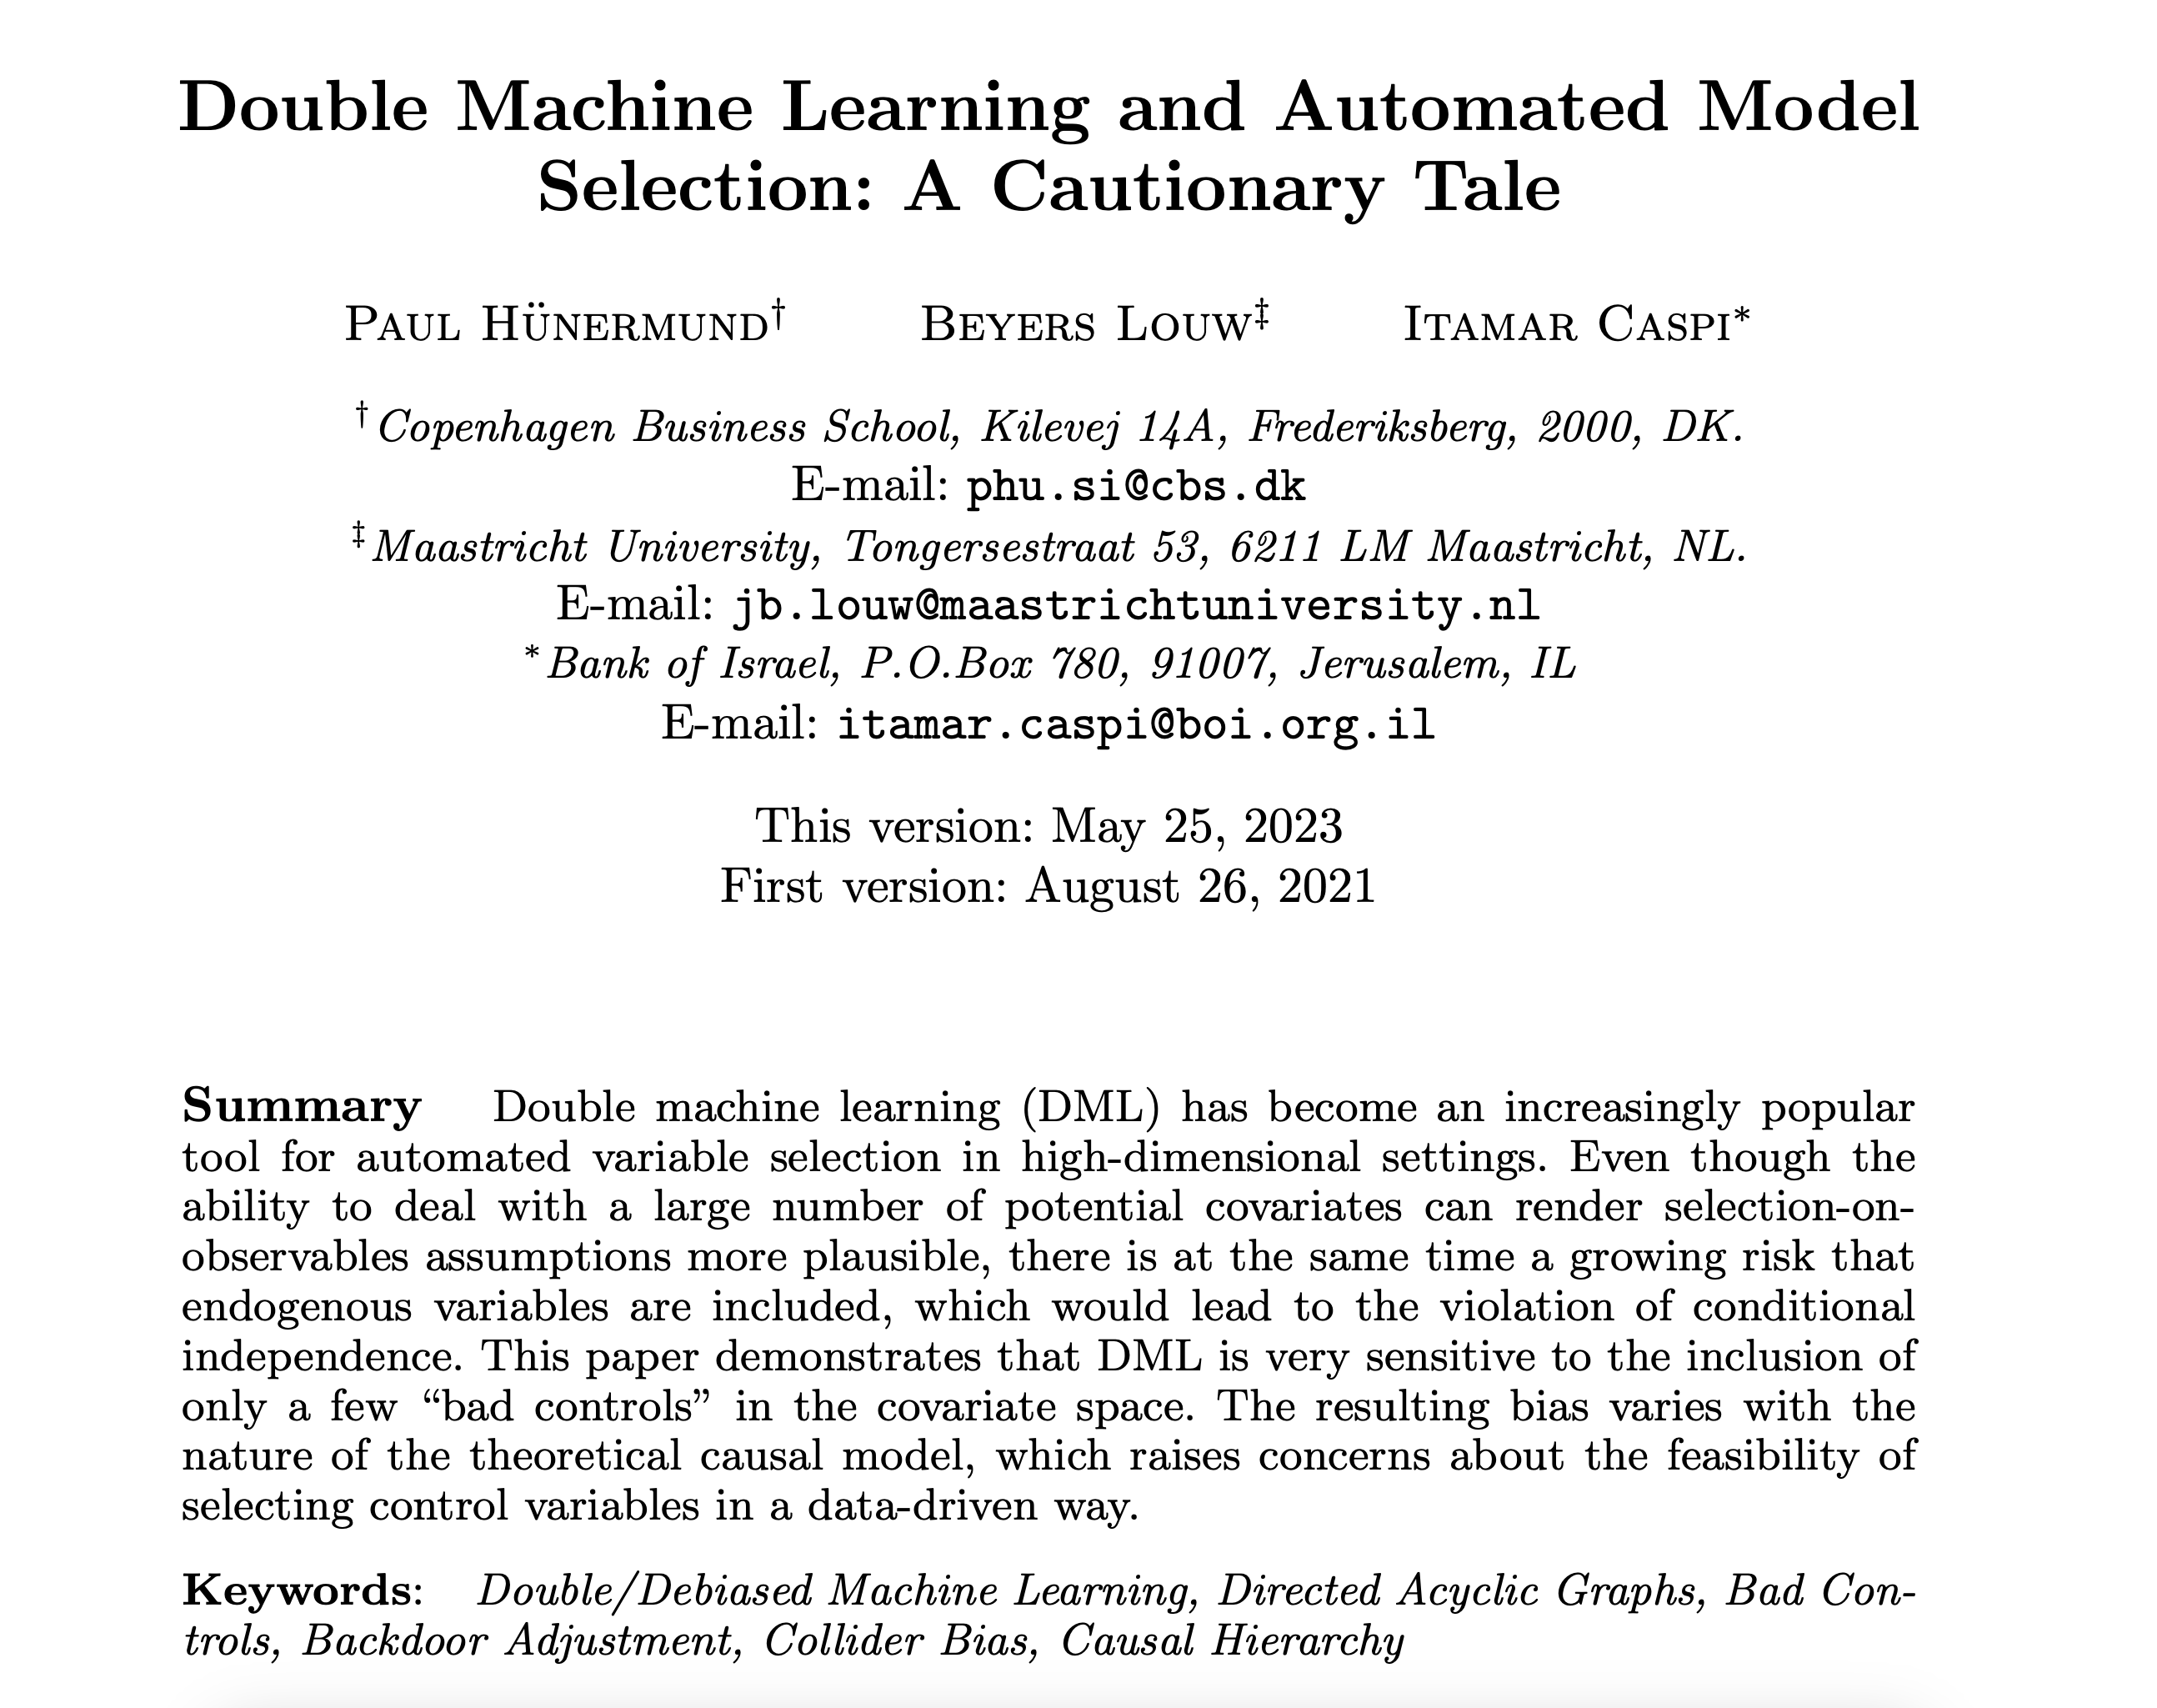
\includegraphics[scale=0.25]{./lecture_includes/paul_dml}
  \end{figure}

\end{frame}


\begin{frame}{Contrast this with ordinary practices}

\begin{itemize}
\item Person attempts to ``control for omitted variable bias'' by including as many ``controls'' as possible
\item Person does not even attempt to think about treatment assignment mechanism and therefore has no idea what variables are colliders, covariates or confounders
\end{itemize}

\end{frame}






\end{document}
\begin{frame}{M-bias as collider}



  \centering
  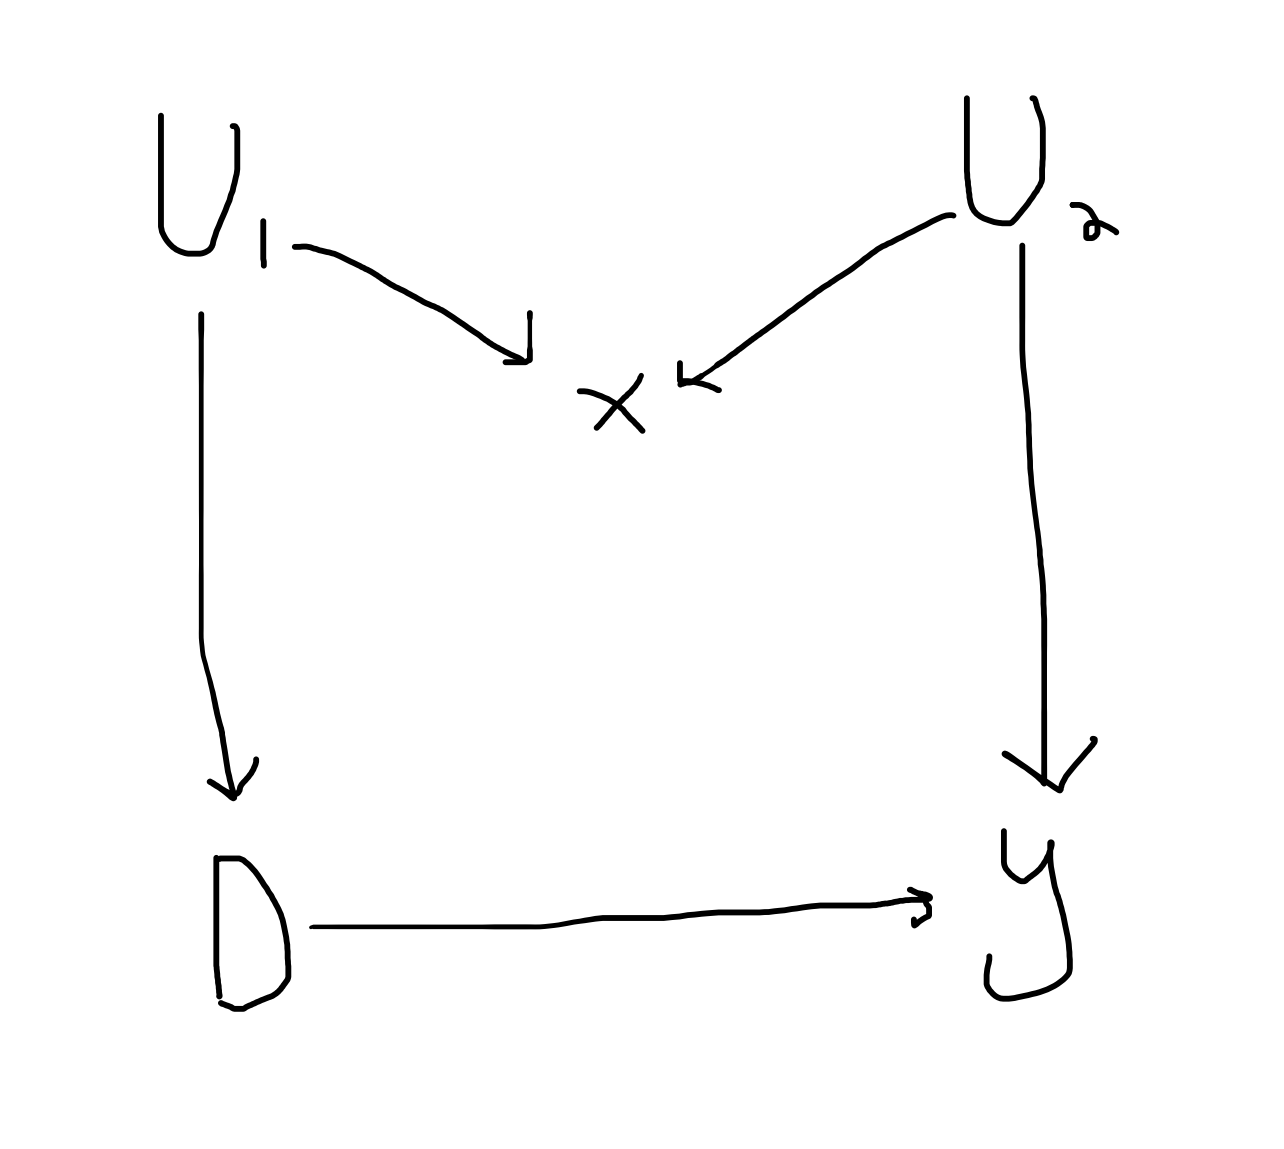
\includegraphics[scale=0.5,height=6.5cm, width=10cm]{./lecture_includes/mbias}

\footnotesize
$X$ is pre-treatment, but if you conditioned on it, then $D\leftarrow U1 \rightarrow \mbox{X} \leftarrow U2 \rightarrow Y$ and $X$ is a collider. Colliders take strange forms, so the conditioning set \emph{must} be thoughtfully chosen based on being a strong predictor of $Y^0$, preferably based on expert knowledge and not a kitchen sink of all available regressors

\end{frame}


